%MEGA MAN X3.TEX

\textit{Mega Man X3} is third installment in the \textit{Mega Man X} series. Released in Japan on December 1st 1995 and later in North America and PAL regions in 1996, Mega Man X3 is the last instance of the series on the SNES console. The game received a second release upgraded to 32-bit for Sony PlayStation and Sega Saturn (in 1996) and for Windows systems (in 1997). This second version came also with Full-motion videos for the opening scene and bosses' introduction, making it the first game of the franchise to have such feature, as well as a newly synthesized soundtrack. Just like its predecessor, X3 too uses the Cx4 graphics Chip for pseudo-3D graphics and transparencies. Since at the time the game was developed Capcom was focusing their effort on developing for PlayStation and Saturn, the game was outsourced to Minakuchi Engineering, who had previously worked on Mega Man's games for the Game Boy and \textit{The Wily Wars} for the Genesis.

\begin{figure}[htp]
	\centering
	\begin{subfigure}[c]{0.4\linewidth}
		\centering
		
\includegraphics[width=\linewidth]{figures/X3/Mmx3_box.jpg}
	\end{subfigure}
	\begin{subfigure}[c]{0.4\linewidth}
		\centering
		
\includegraphics[height=5cm]{figures/X3/X3_ps.jpg}
	\end{subfigure}
	\caption{Cover art for the SNES and Play Station version of the game.}
\end{figure}

\section{Main plot}
After an unspecified amount of time from the previous game's events, Sigma's rebellion has finally been stopped thanks to the effort of X, Zero and the Maverick Hunters. Despite this success, Maverick attacks had continued to happen, forcing the Hunter to intervene. It is only thanks to the genius of the reploid scientist Dr.~Doppler that the cause of maverick's apparitions is discovered in a computer virus which force a reploid to go maverick. Dr.~Doppler names this particular virus the Sigma Virus, and immediately begins to create a countermeasure for it. Thanks to his efforts the virus is  finally  stopped and infected reploids returned normal, seemingly halting the mavericks for good.  Following such success, many reploids gathered around their savior DR.~Doppler, resulting in the foundation of what Doppler Town, a perfect Utopian community where humans and reploids live together. At this point in time, the situation seem to turn for the better, with the world entering a new golden age led by Doppler's achievements.

\begin{figure}[htp]
	\centering
	
\includegraphics[width=.6\linewidth]{figures/X3/Story_1.jpg}
	\caption{X and Zero dispatching against Doppler}
\end{figure}
Such situation, however, last only for a few months. After this amount of time, in fact, reploids whose maverick behavior was supposed to be suppressed suddenly began to riot, revealing that the ``vaccine'' developed by Doppler was merely a placebo. Because of this, the scientist is appointed as responsible for the riot and Maverick Hunter are ordered to arrest him. X and Zero are then dispatched to infiltrate Doppler Town and capture him but, few hours after their intrusion, Doppler's forces begin attacking the Maverick Hunters HQ, forcing the two to quickly return and defend their base. During such operation former Hunter and now Doppler's follower Mac betrays and captures X, only to be later destroyed by Zero coming to rescue his friend. Together the two friends manages to save the HQ from the attack, and then resume their mission of capturing Doppler. The two proceed to fight against the eight mavericks, as well as the two other forces Doppler send to halt the couple: the Nightmare Police, constituted by Doppler's creation Bit and Byte, as well as a revived and vengeful Vile, now upgraded to Vile Mk-II. However neither them nor the mavericks manage to halt X and Zero which, with the help of Dr.~Cain, locate Doppler's laboratory and proceed to raid it.
\begin{figure}[htp]
	\centering
	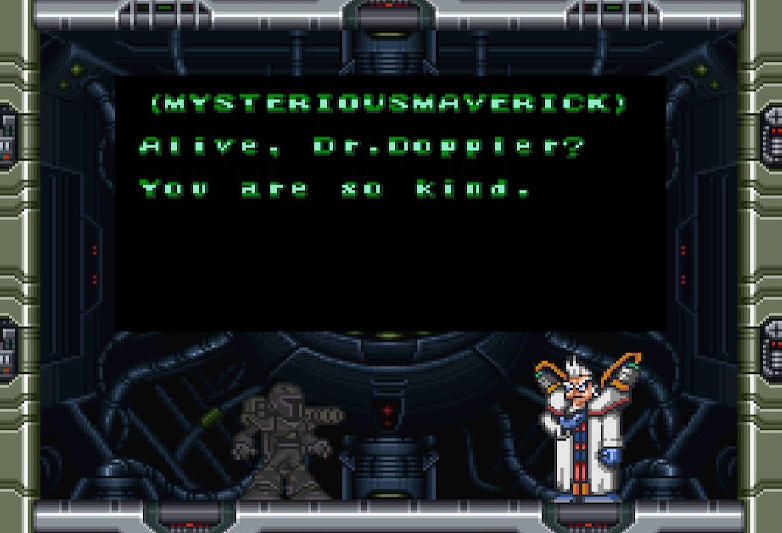
\includegraphics[height=4cm]{figures/X3/Story_2.jpg}
	\caption{Doppler and a ``misterious'' maverick}
\end{figure} Dr.Cain also warns X that, according to his studies, Doppler has used the riot to gather information on latest models of reploid in order to create a new powerful body. X and Zero manages to reach the deepest part od Doppler's hideout, where they finally met with the scientist, which in the meanwhile as upgraded his body to a one more suitable for battle. X and Doppler proceed to fight, but the scientist is no match for the hunter, which easily win the fight. Once defeated, Doppler regain his senses, revealing the truth behind all his doing: it was Sigma who had maneuvered the scientist's action all along, having infected him from the very beginning. Doppler then warns X about the new body he had built for Sigma, and asks him to stop Sigma one again. X proceed then to confront with Sigma and his new body, managing to defeat him too. In a final attempt to claim victory, Sigma enter in his viral form and chase X to try possessing his body. X escapes but reaches a dead end and is cornered by Sigma. Here two possible endings can play depending on whether Zero is damaged or not. In the latter case, he will appear behind Sigma and hit him with his Z-saber upgraded with an antivirus created by Doppler, which will cause Sigma to disappear. In the second case instead it will be Doppler, which as regain control over his body, to inject the antivirus into Sigma, by leaping onto him. This will again cause Sigma to disappear, but this time at the cost of Doppler's life.

Whatever the scenario, after Sigma's defeat, X and Zero will meet outside Doppler's lab now in ruin, pondering again on the fate of reploids and humans and on the reason to fight. However as the dialogue proceed, the narrator dialogue diverge from X's thoughts, revealing the only truth, which is that X and Zero are destined to fight, although no one knows when.

\begin{figure}[htp]
	\centering
	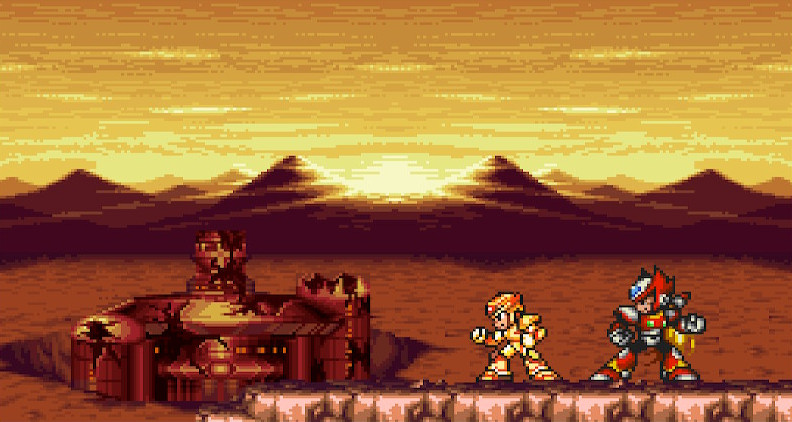
\includegraphics[width=.4\linewidth]{figures/X3/Story_3.jpg}
	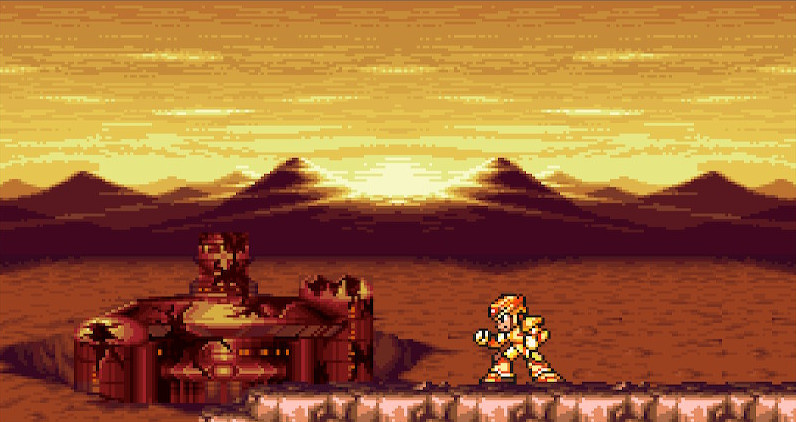
\includegraphics[width=.4\linewidth]{figures/X3/Story_32.jpg}
	\caption{Game's final scene with and without Zero}
\end{figure}

\section{Main Characters}
\subsection{X}
\begin{figure}[htp]
	\centering
	
\includegraphics[height=4cm]{figures/X3/X.png}
	\caption{X as he appears in X3~\cite{book:MMX_Complete_art}.}
\end{figure}
X (more detail in chapter~\ref{char:X}) is the main protagonist of the game. He is the leader of the Maverick Hunters' 17th Elite Unit, and at this point of time he has begun an expert in dealing with Mavericks. However his task of keeping peace often conflicts with his kind heart which repels fighting, causing inside him a struggle only few people can understand.

X's origins are still considered a mystery, and event the latest technology of 22nd Century cannot totally analyze X's full potential~\cite{Xcoll1:Manual_X3}.

\subsection{Zero}
\begin{figure}[htp]
	\centering
	
\includegraphics[height=4cm]{figures/X3/Zero.png}
	\caption{Zero as he appears in X3~\cite{book:MMX_Complete_art}.}
\end{figure}
Zero (full details in chapter\ref{char:Zero}) is an SA-class maverick hunter, as well as the leader of the Special 0th Unit, after being repaired after the events of the precedent game. He act as a mentor and a friend for X, having spent years fighting alongside him. Zero is renowned for his cold and professional attitude, never wasting time during a mission. In truth however Zero hides inside a deep hate for all mavericks which X does not share~\cite{Xcoll1:Manual_X3}.

\section{Game Mechanics}
As the third entry in the series, Mega Man X3 borrows many features from its predecessors, although not all of them, while also adding new features to keep the gameplay fresh:
\begin{itemize}
	\item Stage interaction returns from the first game: Now beating a stage will effect one ore more other stages making easier their navigation by removing some potential danger, unlocking new paths or making enemies weaker.
	\item The Ride Armor system has been updated. Ride Armors now are summoned in from specific platforms found in the stages. New types of Ride Armor can be piloted, but in order to unlock them their modules have first to be found. Once unlocked, a Ride Armor can be summoned anywhere a platform can be found.
	\item Alongside traditional Armor Parts, new Pink capsules can be found too. Such capsules, hidden in stages, contains an upgrade chip for one of X's armor parts and can enhance this upgrade even more. Clearly an upgrade chip can only be obtained if X already possesses the corresponding armor part and, moreover, it is possible to obtain only one upgrade chip throughout the entire game, as the enhancement is permanent and only one can be collected.
	\item The Ride Chasers are not more present in the game.
	\item Throughout an option in the pause menu, Zero can become playable, although with some limitations. More information about this feature are given in section~\ref{X3:Zero}
	\item Nightmare Police challenges: Much similar to the X-Hunters from the previous game, after a certain number of bosses have been defeated the Nightmare police will begin spawning in the stage to challenge X. Differently from the previous game, however, only one boss will spawn at the time, Bit appearing after defeating two bosses and Byte after five. Additionally, purposely avoiding the fight is not possible anymore, as their boss rooms are placed in middle of the stages without any possibility to avoid them. When X enters one of these rooms, the boss fight will trigger randomly each time, and even between two subsequent visit following a defeat
	\item Vile stage: After the Nightmare Police begins chasing X, in specific stages a teleporter pad will also appears. Such teleporter, once taken, brings X into the Vile stage, where players can challenge Vile himself.
\end{itemize}
\section{Weapons}\label{X3:sub_weapon}
\subsection{
\includegraphics[width=12px, height=10px]{figures/X3/weapons/A_burst.jpg} Acid Burst}\label{Acid_Burst}
Acid Burst allow X to shoot a glob of acid which damages enemies. Upon making contact with a surface, the bubble explodes into four small acid drops which deal less damage but cover a wider area. This weapon can also be aimed, by inputting the UP or DOWN command as soon as the fire button is pressed, to shoot the bubble straight up or down. When charged this weapon will release two acid balls which bounce forward five times before disappearing. Since the acid burst is a liquid weapon, firing it underwater will immediately dissipate the bubble, making this weapon useless in this condition. 

This weapon also posses the useful ability to guarantee weapon energy drop when defeating following enemies~\cite{X3:enem_drop_gfaqs}:
\begin{itemize}
	\item \hyperlink{enem:Atareeter}{Atareeter}
	\item \hyperlink{enem:Blady}{Blady}
	\item \hyperlink{enem:Crablaster}{Crablaster}
	\item \hyperlink{enem:Drimole-W}{Drimole-W }
	\item \hyperlink{enem:Ganseki_Carrier}{Ganseki Carrier}
	\item \hyperlink{enem:Hamma_Hamma}{Hamma Hamma}
	\item \hyperlink{enem:Head_Gunner_customer}{Head Gunner customer} \& \hyperlink{enem:Head_Gunner_masspro}{Head Gunner masspro}
	\item \hyperlink{enem:Meta_Capsule}{Meta Capsule}
	\item \hyperlink{enem:Notor_Banger}{Notor Banger}
	\item \hyperlink{enem:Tombort}{Tombort}
	\item \hyperlink{enem:Victoroid}{Victoroid} \& \hyperlink{enem:Victoroid_customer}{Victoroid customer}
	\item \hyperlink{enem:Walk Blaster}{Walk Blaster}
\end{itemize}

To obtain the Acid Burst X as first do fight and defeat Toxic Seahorse (\ref{boss:Toxic_seahorse}) in his stage.

\begin{figure}[htp]
	\centering
	\begin{subfigure}{3.9cm}
		
\includegraphics[height=2.7cm]{figures/X3/weapons/A_burst.png}
		\caption{Normal fire}	
	\end{subfigure}
	\begin{subfigure}{3.9cm}
		
\includegraphics[height=2.7cm]{figures/X3/weapons/A_burst_up.png}	
		\caption{Up fire}
	\end{subfigure}
	\begin{subfigure}{3.9cm}
		
\includegraphics[height=2.7cm]{figures/X3/weapons/A_burst_Down.png}	
		\caption{Down fire}
	\end{subfigure}
	\begin{subfigure}{0.4\linewidth}
		\centering
		
\includegraphics[height=2.7cm]{figures/X3/weapons/A_burst_charge.png}
		\caption{Charged version}	
	\end{subfigure}
	\begin{subfigure}{0.4\linewidth}
		\centering
		
\includegraphics[height=2.7cm]{figures/X3/weapons/A_burst_water.png}
		\caption{Underwater.}
	\end{subfigure}
	\caption{Acid Burst sub-weapon}
\end{figure}


\subsection{
\includegraphics[width=12px, height=10px]{figures/X3/weapons/P_bomb.jpg} Parasitic Bomb}\label{Parasitic_Bomb}

Upon defeating Blast Hornet~\ref{boss:Blast_hornet}, X will add the Parasitic Bomb to his arsenal. Upon pressing the fire button this weapon will launch a spiked bomb forward which will result in either two scenarios upon making contact with an enemy. If the enemy is of large size, the bomb will simply explode to deal damage; if, however, the enemy is of small size the bomb will latch onto it, paralyzing and keeping it in stasis. An enemy in this status is essentially neutralized, as it cannot neither attack or deal contact damage to X. Upon blocking an enemy, the Parasitic Bomb will then make one of the following actions: If no other enemies are nearby it will explode alongside the trapped enemy; otherwise the bomb and its victim will home onto the nearest enemy, exploding as soon as they make contact. 

The charged version of this weapon is rather peculiar. Upon charging, four cursors will surround X and remain in position until an enemy comes nearby. At this point the nearest cursor will lock onto it and X will fire a robotic hornet to such enemy. Once the hornet explodes another cursor will appear around X to replace the one which aimed at the enemy. The peculiarity reside in two elements. First, the charged version of the weapon will last until the fire button is pressed, meaning that the cursors will remain on screen up until this button is pressed, and releasing it will stop the ``charge'' status of the weapon. Secondly, differently from other weapons which keep draining energy while active, the charged version will use ammunition only when a hornet is fired, and it does not require energy to maintain the charge.

\begin{figure}[htp]
	\centering
	\begin{subfigure}{.49\linewidth}
		\centering
		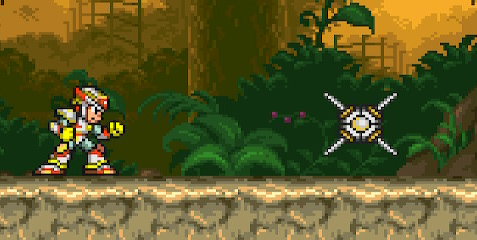
\includegraphics[height=3cm]{figures/X3/weapons/P_bomb.png}
		\caption{Normal fire}	
	\end{subfigure}
	\begin{subfigure}{.49\linewidth}
		\centering
		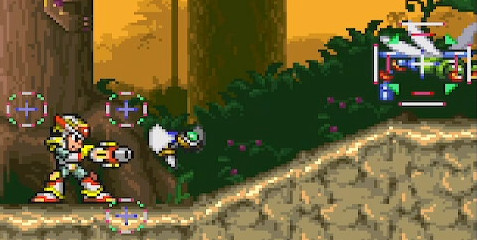
\includegraphics[height=3cm]{figures/X3/weapons/P_bomb_C.jpg}
		\caption{Charged version}	
	\end{subfigure}
	\caption{Parasitic Bomb sub-weapon}
\end{figure}


\subsection{
\includegraphics[width=12px, height=10px]{figures/X3/weapons/T_thunder.jpg} Triad Thunder}\label{Triad_Thunder}

The Triad Thunder is the weapon X obtains by defeating Volt Catfish~\ref{boss:Volt_catfish}. This sub-weapon generates three orbs around X in a triangular pattern which conducts electricity, forming a sort of shield. After few seconds the three orbs will fire stored electricity in their respective direction (up, diagonal-down left and diagonal-down right) and will then fall off-screen. It is possible, if the player has the right timing, to swap the orbs' position to form an upside-down triangle. With the correct timing it is also possible re-change the position to its original state, but it is important to note that for each change weapon ammunition is used. When charged X will punch the ground to release a shockwave which will deal massive damage to all enemies touching it. Moreover after the initial shockwave two electric sparks will part from X moving in opposite directions and following the ground.

\begin{figure}[htp]
	\centering
	\begin{subfigure}{3.9cm}
		\centering
		
\includegraphics[height=3.5cm]{figures/X3/weapons/T_thunder.png}
		\caption{Normal fire}	
	\end{subfigure}
	\begin{subfigure}{3.9cm}
		\centering
		
\includegraphics[height=3.5cm]{figures/X3/weapons/T_thunder_3.png}
		\caption{Releasing electricity}	
	\end{subfigure}
	\begin{subfigure}{3.9cm}
		\centering
		
\includegraphics[height=3.5cm]{figures/X3/weapons/T_thunder_2.png}
		\caption{Upside-down formation}	
	\end{subfigure}
	\begin{subfigure}{\linewidth}
		\centering
		
\includegraphics[height=3.5cm]{figures/X3/weapons/T_thunder_C.png}
		\caption{Charged version}	
	\end{subfigure}
	\caption{Triad Thunder sub-weapon}
\end{figure}

\subsection{
\includegraphics[width=12px, height=10px]{figures/X3/weapons/S_blade.jpg} Spinning Blade}\label{Spinning_Blade}
When equipping this sub-weapon, the X buster will fire two spinning blade which travel forward for short amount of time, before curving backwards, one with an upward direction and the second downward. Due the particular trajectory of this weapon, using this weapon may result difficult at first, as its main use is to hit enemies behind X. However this weapon can also be used at close range in a shotgun-like way to make both blade hit a single enemy to deal massive damages. 
Upon charging, this weapon will release blade in a yo-yo style which will remain at a fixed distance from X as he moves. Upon pressing the UP or DOWN the blade will rotate in the  corresponding direction before returning to its original position. If while spinning the blade makes contact with an enemy it cannot destroy, the blade will bounce off, separating from the X-buster in the process.
This weapon is obtained after defeating Crush Crawfish (\ref{boss:Crush_crawfish}).

\begin{figure}[htp]
	\centering
	\begin{subfigure}{\linewidth}
		\centering
		
\includegraphics[height=3cm]{figures/X3/weapons/S_blade.png}
		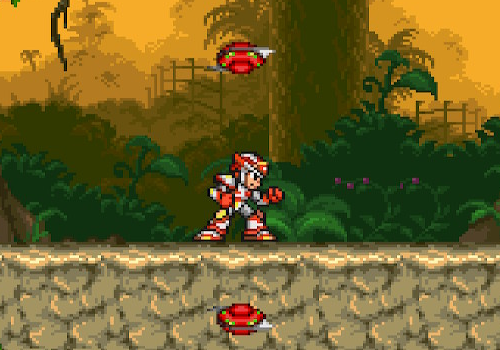
\includegraphics[height=3cm]{figures/X3/weapons/S_blade_1.png}
		\caption{Normal fire }	
	\end{subfigure}
	\begin{subfigure}{\linewidth}
		\centering
		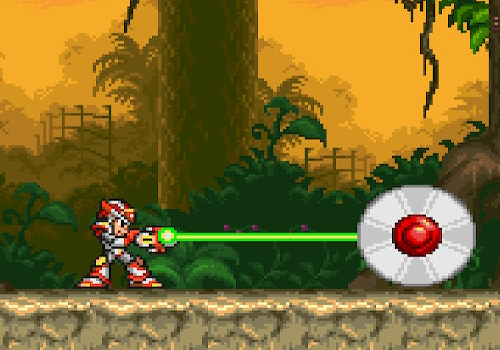
\includegraphics[height=3cm]{figures/X3/weapons/S_blade_C.png}
		
\includegraphics[height=3cm]{figures/X3/weapons/S_blade_C1.png}
		\caption{Charged version}	
	\end{subfigure}
	\caption{Spinning Blade sub-weapon}
\end{figure}

\subsection{
\includegraphics[width=12px, height=10px]{figures/X3/weapons/R_splasher.jpg} Ray Splasher}\label{Ray_Splasher}
The Ray Splasher is the weapon X obtains after defeating Neon Tiger (\ref{boss:Neon_tiger}). When using this weapon X will fire a volley of energy bullet in a spread formation. Upon charging this weapon X will release a glass container in the sky, which will shoot twenty-two Ray Splasher bullets in random direction.
\begin{figure}[htp]
	\centering
	\begin{subfigure}{.3\linewidth}
		\centering
		
\includegraphics[height=3cm]{figures/X3/weapons/R_splasher.png}
		\caption{Normal fire}	
	\end{subfigure}
	\begin{subfigure}{.3\linewidth}
		\centering
		
\includegraphics[height=3cm]{figures/X3/weapons/R_splasher_C.png}
		\caption{Charged version}	
	\end{subfigure}
	\caption{Ray Splasher sub-weapon}
\end{figure}
\subsection{
\includegraphics[width=12px, height=10px]{figures/X3/weapons/G_well.jpg} Gravity Well}\label{Gravity_Well}
When equipped with this sub-weapon, X will shoot a floating device which travels for a short distance before halting and activating a small high-gravity around it. Weak enemies which happen to be inside this area are instantly destroyed, while other enemies will remain untouched. After a few seconds the device will stop working and will return to X, which cannot fire another one until the first has returned. When charged, X will release a small black hole upwards, which will cause the gravity to shift up, carrying all weak enemies on screen alongside it. This weapon is acquired by X after defeating Gravity Beetle (\ref{boss:Gravity_beetle}). 
\begin{figure}[htp]
	\centering
	\begin{subfigure}{.25\linewidth}
		\centering
		
\includegraphics[height=3cm]{figures/X3/weapons/G_well.png}
		\caption{Normal fire}	
	\end{subfigure}
	\begin{subfigure}{.6\linewidth}
		\centering
		
\includegraphics[height=3cm]{figures/X3/weapons/G_well_C.png}
		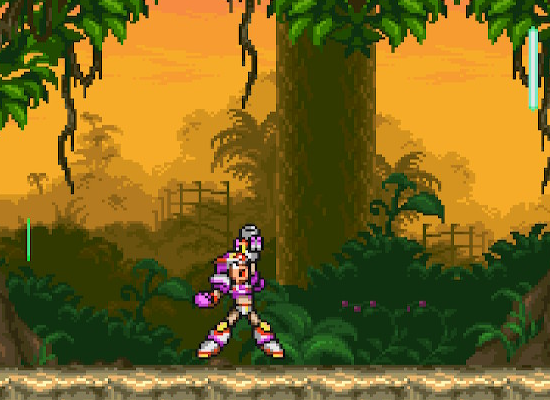
\includegraphics[height=3cm]{figures/X3/weapons/G_well_C_1.png}
		\caption{Charged version}	
	\end{subfigure}
	\caption{Gravity Well sub-weapon}
\end{figure}
Enemies immediately destroyed by this weapon are~\cite{wiki:damage_chart_X3}:
\begin{itemize}
	\item \hyperlink{enem:Blady}{Blady}
	\item \hyperlink{enem:Caterkiller}{Caterkiller}
	\item \hyperlink{enem:Earth_Commander}{Earth Commander}
	\item \hyperlink{enem:Ganseki_Carrier}{Ganseki Carrier}
	\item \hyperlink{enem:Helit}{Helit}
	\item \hyperlink{enem:Mine_Tortoise}{Mine Tortoise}
	\item \hyperlink{enem:Notor_Banger}{Notor Banger}
	\item \hyperlink{enem:Tombort}{Tombort}
	\item \hyperlink{enem:Wall_Cancer}{Wall Cancer}
\end{itemize}
\subsection{
\includegraphics[width=12px, height=10px]{figures/X3/weapons/F_shield.jpg} Frost Shield}\label{Frost_Shield}
Upon defeating Blizzard Buffalo (\ref{boss:Blizzard_buffalo}), X will gain access to the Frost Shield. When fired, this weapon will create a small icicle missile which moves forward after an initial delay. Upon making contact with a wall or an enemy the projectile will bounce off, creating a three-spiked trap on the ground which remain in position for few seconds before disappearing. X can fire up to two missiles at the time, but has to wait for the spikes to disappear before firing a third one. Upon charging X will create a spiked block of ice at the end of his X-buster which will deal damage to enemies which make contact with it and also acting as an effective shield, blocking incoming projectiles. After about nine seconds the shield will shatter and what remain will slide across the ground, but if X performs an air-dash the shield will immediately destroy.

When used underwater, the effects of this weapon change slightly: for the normal fire the missiles and spikes will have their size doubled, while the charged version replace the spiked shield with an ice boulder which float towards the surface and where X can stand on.

Finally, just like the Acid Burst (\ref{Acid_Burst}), this weapon too has the perks to guarantee health drop when destroying certain enemies (the same for which Acid Burst drops Ammo pickup), making it very effective for sub-tank filling.

\begin{figure}[htp]
	\centering
	\begin{subfigure}{3.9cm}
		\centering
		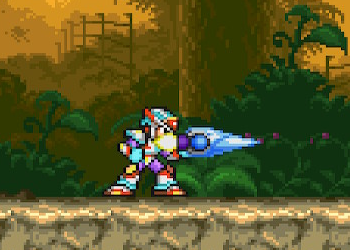
\includegraphics[height=2.7cm]{figures/X3/weapons/F_shield.png}
		\caption{Icicle Missile}	
	\end{subfigure}
	\begin{subfigure}{3.9cm}
		\centering
		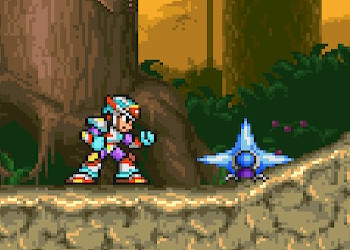
\includegraphics[height=2.7cm]{figures/X3/weapons/F_shield_1.jpg}
		\caption{Ice spike}	
	\end{subfigure}
	\begin{subfigure}{3.9cm}
		\centering
		
\includegraphics[height=2.7cm]{figures/X3/weapons/F_shield_C.png}
		\caption{Charged version}	
	\end{subfigure}
	\begin{subfigure}{3.9cm}
		\centering
		
\includegraphics[height=2.7cm]{figures/X3/weapons/F_shield_C_1.png}
		\caption{Shield remains sliding}	
	\end{subfigure}
	\begin{subfigure}{3.9cm}
		\centering
		
\includegraphics[height=2.7cm]{figures/X3/weapons/F_shield_C_2.png}
		\caption{Charged underwater }	
	\end{subfigure}
	\begin{subfigure}{3.9cm}
		\centering
		
\includegraphics[height=2.7cm]{figures/X3/weapons/F_shield_C_3.png}
		\caption{Using as a platform}	
	\end{subfigure}
	\caption{Frost Shield sub-weapon}
\end{figure}
%TODO picture of undwewater spikes

\subsection{
\includegraphics[width=12px, height=10px]{figures/X3/weapons/T_fang.jpg} Tornado Fang}\label{Tornado_Fang}
After defeating Tunnel Rhino (\ref{boss:Tunnel_rhino}),X will adapt the Tornado Fang into his arsenal. When used this weapon will fire a drill-shaped missile which briefly delays (just like the Frost Shield) before starting to move. Upon pressing the fire button again while the drill is stationary two more missiles can be spawned, for a total of three. Upon making contact with an enemy the missile will try to perforate the enemy, dealing constant damage in the process until its charge is depleted. If it successfully destroys an enemy it will keep moving forward until its charge is depleted. When charged this sub-weapon changes the X-buster into a drill until the fire button is pressed. While in this state X will deal damage to all enemies which make contact with it and, furthermore, the drill will also stick to the wall when X is wall jumping, allowing him to stay in place without sliding down.

\begin{figure}[htp]
	\centering
	\begin{subfigure}{\linewidth}
		\centering
		
\includegraphics[height=3cm]{figures/X3/weapons/T_fang.png}
		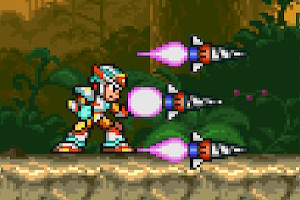
\includegraphics[height=3cm]{figures/X3/weapons/T_fang_1.png}
		\caption{Normal fire }	
	\end{subfigure}
	\begin{subfigure}{\linewidth}
		\centering
		
\includegraphics[height=3cm]{figures/X3/weapons/T_fang_C.png}
		
\includegraphics[height=3cm]{figures/X3/weapons/T_fang_C_1.png}
		\caption{Charged version + sticking to a wall}	
	\end{subfigure}
	\caption{Tornado Fang sub-weapon}
\end{figure}

\section{Third Armor + Beam-saber}\label{X3:Armor}

Following the trend of its predecessors, Mega Man X3 too offers to players a way to increase X's power through the usage of Armor Parts. This time, however, four more capsules can be found, bringing the total of hidden pieces up to eight, on per stage. Such additional capsules, painted in pink to distinguish them to regular ones, however do not contain actual armor parts but rather augment chip for a specific armor piece, which must be acquired first in order to obtain the power-up. The trade-off for such augment is, however, that the armor can only stand one of them and that they cannot be replaced, making the chosen upgrade permanent for the entire game. However, continuing the tradition of previous games, a final hidden capsule can be obtained as a prize for obtaining all collectible in the game, safe for said additional capsule. Such last capsule will give the player a special armor upgrade, which combines all the four optional chips into a single one, while also changing the armor color to gold. Finally, although not directly a part of the armor, there is another hidden upgrade X can obtain regardless of the armor status: the Beam-Saber

The Third armor (also known as Max Armor~\cite{wiki:third_armor}) is composed by the following parts:
\begin{itemize}
	\item Foot parts: Found in 	the Frozen Town Stage, near the end of the large area before the boss' room. This upgrade allows X to regain the air-dash ability in the same way as it was for the second armor. This time however the air dash can also be performed upwards, although with a short delay between the first and second jump. Just like the previous game, X cannot air-dash out of a dash-jump. It is possible, however, perform two upward dash, as it is not required for X to touch the ground before performing a second one.
	
	
	\item Body Parts: Just like its predecessor, this part double X's defense by cutting in half all incoming damages. In addition, when X receives damage a blue force field appears around X for a short amount of time, reducing incoming damage for an additional 25\%, for a total damage reduction of 62.5\%. This upgrade is found in Volt Catfish's stage, on the vertical spiked pit after the fourth lift. It requires either a charged Gravity Well to lift the platform or the Foot Part with the upgrade chip (although it is not mandatory as it is possible to reach the upper ledge by combining two well timed upward dash).
	
	\begin{figure}[htp]
		\centering
		
\includegraphics[height=3cm]{figures/X3/weapons/Armor_shield.png}
		\caption{Shield activated}
	\end{figure}
	
	\item Arm Parts: Increase X's maximum charge level up to four, while also allowing to charge sub-weapons. Similarly to he Second Armor, releasing a fully charged shot will cause X to shoot a single shot, while keeping a second one in store for later. It is also possible to release the second shot immediately after the second, just like in X2, but in this case the two shots instead of moving separately will combine in a single Cross Charged Shot. Although powerful, this attack also comes with some drawbacks, mainly the delay the two shots need to combine and start moving, which can cause to miss some potential opening in the enemies. 
	Beside the increase in attack power, the Arm Parts also X's to move faster on ladders, as well as cutting the ammo cost for sub-weapon in half, but only when the armor is fully completed. This part can be found in the Safari Park, behind a wall breakable by the Tornado Fang and a pit which requires a double dash to pass on.
		
	\begin{figure}[htp]
		\centering
		
\includegraphics[height=3cm]{figures/X3/weapons/Combo_shot.png}
		\caption{Cross charged shot}
	\end{figure}
	
	\item Head Parts: Found in Tunnel Rhino's stage, in a path opened by a boulder fall after using the charged Triad Thunder. This parts will add a radar to X's equipment which will map the current stage's layout and point out yet-to-discover collectibles, such as other armor capsule, life-up and sub-tanks. The map is displayed only once as soon as X enters a stage, but it requires an input for the player to close, so it can remain on screen for as much as the player wants. Additionally, on the stage selection screen additional information for each stage will be displayed, showing collectibles for each stage and highlighting missed ones.
		
	\begin{figure}[htp]
		\centering
		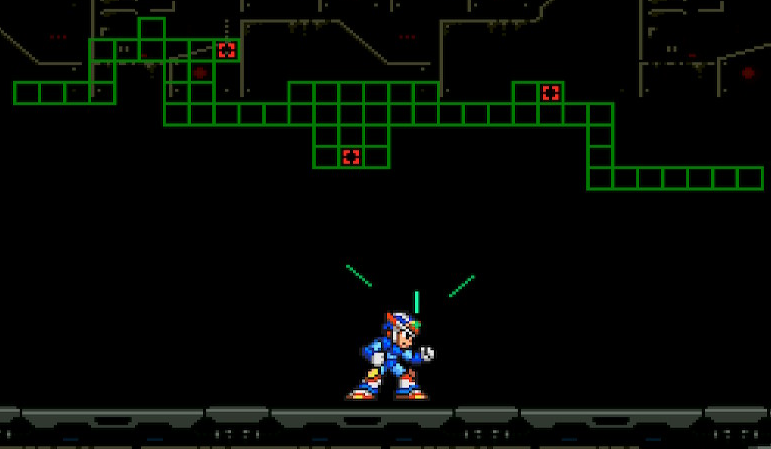
\includegraphics[height=3cm]{figures/X3/Blast_hornet/map.png}
		\caption{Map layout displayed}
	\end{figure}
	
\end{itemize}

As said previously, for each part an upgrade chip can be installed. Hence there are four total chip upgrades, plus a hidden fifth one. the chips are the following:
\begin{itemize}
	\item Foot Chip: Found in Toxic Seahorse's stage, on the surface of the big underwater room on the right. It requires either the charged Frost Shield to reach the surface and jump from there or the Frog Ride Armor, to destroy the fans which prevent X to wall jump on the rightmost wall. The Chip allows X to perform a second air dash in any direction, or an air-dash out of a dash-jump.

	\item Body Chip: Increase the power of the force field emitted by the part after receiving a hit. The shield now becomes orange, and cut damages by another 50\%, for a total of 75\% damage reduced. This chip can be found in the Shipyard stage, in a passage down a pit closed by a wall breakable only by using a Ride Armor.

%TODO orange shield
	\item Arm Chip: Allows the usage of the Hyper Charge, which grants unlimited charged shots as long as there is weapon energy available. The chip is found in Gravity Beetle's stage, at the end of a spiked path blocked by crates breakable only by using a Ride Armor.
	
	\item Head Chip: Enable health regeneration when X stand still. When X remain standing for a while his health will begin to regenerate and the regeneration will continue for as long as he doesn't move. If X is at full health, the regeneration effect will replenish his sub-tanks instead. This chip is found in the Weapons Factory Stage, at top-right side of the area past the elevator, accessible by using the Falcon Module for the Ride Armor.
	
	\item Hyper Chip: Obtainable only if X has obtained all the collectibles and has not installed any other chip. Once obtained, X's armor turns gold and X gets access to all the previous upgrades, with the addition of having an increased health regeneration and a less usage of energy when in Hyper Charge. The capsule for the chip is hidden in Doppler Stage A, in a secret room inside a pit but only if the player reaches it at full health. This upgrade is NOT saved by the password system.
	%TODO better hyper chip screenshot 
\end{itemize}
The last upgrade X can obtain is the beam saber. This upgrade can be obtained independently from the armor's status, as the actions required to obtain it can be done even by regular X. However obtaining this upgrade while also having the Arm Parts will increase its power.

The path which leads to obtain the Beam Saber is rather straightforward, and obtainable with the following steps:
\begin{enumerate}
	\item Find and defeat Vile mk.II using one of his weakness, killing him in the process.
	\item By killing Vile, the Doppler Stage B will change accordingly. In the new path X will find the sub-boss  \hyperlink{miniboss:Mosquittus}{Mosquittus}. This is the only sub-boss Zero can fight and, upon defeating it, the boss will self-destruct after trapping him. This will cause Zero to be seriously damaged (preventing him to be called again) but in exchange he will give X his Beam Saber.
\end{enumerate} 
The Beam Saber gives X another level in his charge shot, which turns green. Upon releasing the fire button, X will swing the beam saber dealing massive damage to every enemy he hits with it. If X is equipped with the Arm Part, the saber will also produce a shockwave which travels forward, and upon making contact with an enemy will not only deal heavy damages to the target, but also produce three more slashes which will deal even more damage over time. In particular, hitting any enemy with the saber itself will deal 30 damage per frame to all enemies whereas a fully charged saber will deal a total of 98 damages. When fighting bosses, the regular saber will deal 16 damages (half health bar), while the shockwave will deal 8 damages, followed by three slashes which deals 4 damages each, dealing in total 20 damages.

\begin{figure}[htp] 
	\centering
	
\includegraphics[height=3cm]{figures/X3/weapons/Z_saber_1.png}
	\includegraphics[height=3cm]{figures/X3/weapons/Z_saber_2.png}
	\caption{Z-Saber swing and shockwave}
\end{figure}

\section{Zero Change}\label{X3:Zero}
A new feature added to the game is the Zero change~\cite{wiki:Zero_change}, which gives the player the ability to play temporary as Zero. From the pause menu, by pressing the L button a secondary screen will appear which can be used to call for Zero. If the player decides to deploy him, Zero will replace X and become playable. 
\begin{figure}[htp] 
	\centering
	\includegraphics[width=.5\linewidth]{figures/X3/weapons/Zero_screen.png}
	\caption{Zero change menu}
\end{figure}
There are, however, some restriction on when Zero can be used:
\begin{itemize}
	\item Zero can only deployed once per stage. If X switches back in, for any reasons, it is impossible to switch again to Zero until the player gets a game over or exits the stage.
	\item Zero cannot engage fight with any bosses or sub-bosses, except for Mosquittus. Upon reaching a boss door, the game will automatically swap back to X.
	\item If Zero dies for any reason, he will become unusable for the rest of the game.
\end{itemize}

Generally speaking, Zero plays similarly to X, but sacrificing defenses for more firepower. Zero in fact, despite possessing more HP than X even after all upgrades are obtained, does not possess any armor upgrade, meaning that enemies will always do full damage to him and depleting his HP quicker than X. In terms of firepower, the Z-buster Zero comes with behave very similarly to the Arm Parts of the third armor, Z-saber included. Zero can charge his shots up to five level, the latter being the saber swing, but the lack of access to sub-weapons greatly limit his fighting options. Also since Zero is a little taller than X, his shots will also be higher. Finally as Zero the player is not able to obtain any collectible, nor can use ride armors.


\begin{figure}[htp]
	\centering
	\begin{subfigure}{\linewidth}
		\centering
		\includegraphics[width=.4\linewidth]{figures/X3/weapons/zero_shot_1.png}
		\includegraphics[width=.4\linewidth]{figures/X3/weapons/zero_shot_2.png}
	\end{subfigure}
	\begin{subfigure}{\linewidth}
		\centering
		\includegraphics[width=.4\linewidth]{figures/X3/weapons/zero_shot_3.png}
		\includegraphics[width=.4\linewidth]{figures/X3/weapons/zero_shot_4.png}
		\caption{Charged version + sticking to a wall}	
	\end{subfigure}
\begin{subfigure}{\linewidth}
	\centering
	\includegraphics[width=.5\linewidth]{figures/X3/weapons/zero_shot_5.png}
\end{subfigure}
	\caption{Zero's charged shots levels.}
\end{figure}

\section{Ride Armors}
A mechanic so far unique to this game is the possibility to unlock and use different types of Ride Armor by summoning them from specific pedestals, known as \textit{Robot Ride platform}~\cite{X3:Manual}. From this devices, X can summon any of the already unlocked armors for his own use. Zero however is completely prevented from using them

There are a total of four different type of Ride Armor, which consists in a base form plus three modules to change its form:
\begin{itemize}
	\item \hyperlink{vehicle:Ride_Armor_Chimera}{Chimera Ride Armor}: The base form of the Ride Armor, which behaves similarly to the one from the first installment of the game. It can punch, jump and dash forward. Being the template for all other types, it is mandatory to obtain this model first, by recovering it from Blast's Hornet stage.
	\item \hyperlink{vehicle:Ride_Armor_Kangaroo}{Kangaroo Ride Armor}: Model designed for combat, similar to the Rabbit model from the previous game.  Equipped with spinning claws, it deals more damage than the Chimera Model, while also being capable of performing a  charged attack which releases a long-ranged spiked fist with a chain attached.
	\item \hyperlink{vehicle:Ride_Armor_Hawk}{Hawk Ride Armor}: Model designed for flight, is equipped with a hover fan which allows it to hover and slowly gain height for few seconds if the jump button is kept pressed. Differently from the other versions, this is equipped with a pair of rocket launcher for long-ranged attack.
	\item \hyperlink{vehicle:Ride_Armor_Frog}{Frog Ride Armor}: Ride Armor specialized in underwater combat. While on land this Ride Armor is very lacking, as it can only proceed by hopping forward with short hops (normal walk) or long jumps (dash) and even its fighting capabilities are severally reduced, as the missiles it propels from his cannons curve down. The situation changes when the armor reaches the water. While underwater, in fact, its jump are much higher and is possible even to concatenate up to six~\cite{wiki:Chimera_Armor} jumps. Moreover the torpedo it shoots gain homing capabilities. Finally, it is important to note that this is the only type of armor capable to move underwater, as all the other sink and become unusable.
\end{itemize}

\section{Opening Stage: Hunter Base}\label{X3:intro_stage}
Few hours after X and Zero are dispatched to Doppler Town, dr.~Doppler's army attack directly the Maverick Hunters HQ, forcing the two to quickly retreat to defend their base, which became the first stage of the game. The stage itself is rather straightforward, as its focus on reintroducing the core mechanics of the series. At about one third of the stage X will meet with \hyperlink{miniboss:Mac}{Mac}, a former Maverick Hunter now member of Doppler's army, which betrays captures X. At this point the game introduces for the first time the Zero Change, forcing the player to take control of Zero for the remaining of the stage. Near the stage's end the player will find Mac as a sub-boss, but he can be easily destroyed thanks to Zero's firepower. Once Mac is destroyed  and X freed , the player will regain control of the latter, to reach the end of the stage and face the boss, Mao the Giant.

This stage houses  the following enemies~\cite{wiki:X3_opening}:
\begin{itemize}
	\item \hyperlink{miniboss:Mac}{Mac}
	\item \hyperlink{enem:Hangerter}{Hangerter}
	\item \hyperlink{enem:Notor_Banger}{Notor Banger}
	\item \hyperlink{enem:Head_Gunner_customer}{Head Gunner customer}
	\item \hyperlink{enem:Caterkiller}{Caterkiller}
	\item \hyperlink{enem:Earth_Commander}{Earth Commander}
\end{itemize}

\subsection{Maoh the Giant}\label{boss:Mao_the_giant}
\begin{figure}[htp]
	\centering
	\includegraphics[height=\portraitsize]{figures/X3/maohthegiant.png}
	\caption{Maoh the Giant's artwork~\cite{book:MMX_Complete_art}}
\end{figure}
Similar to the opening stage of X2, X3 also ends first stage with a fight against a giant mechaniloid. Named "Maoh the Giant", this particular mechaniloid belonging to Doppler's army is stated to be the size of an entire building~\cite{wayback:X3_resources} and was dispatched to attack the Maverick Hunters HQ, before X and Zero quickly returned to destroy him. 
%TODO VERTICAL BALL
\begin{figure}[htp]
\centering
\begin{subfigure}{0.4\linewidth}
	\centering
	\includegraphics[height=3cm]{figures/X3/Diagonal_Ball.jpg}
	\caption{Diagonal Iron Ball}
\end{subfigure}
\begin{subfigure}{0.4\linewidth}
	\centering
	\includegraphics[height=3cm]{figures/X3/Diagonal_Ball.jpg}
	\caption{Vertical Iron Ball}
\end{subfigure}
\caption{Maoh the giant's attacks}
\end{figure}
Although colossal, the fight against Maoh the Giant is relatively easy, considering its only way to attack the player it has is to ram the wrecking ball on the arms towards the player either vertically (\emph{Vertical Iron Ball}) or diagonally (\emph{Diagonal Iron Ball}). These  attacks only cause 1 point of damage, and they leave a crater on the impact point, breaking the arena. Luckily for the player these big spike balls are also Maoh weak point, and together with the fact that its attack are relatively slow, it is very easy to bait an attack, dodge it and hit the spike ball with a charged shot.
\begin{table}[htp]
	\centering
	\begin{tabular}[h]{l c}
		\toprule
		\multicolumn{1}{c}{Health}  & 32\\
		\midrule
		\multicolumn{1}{c}{Attack} & \multicolumn{1}{c}{Damage}\\
		Vertical Iron Ball & 1 \\
		Diagonal Iron Ball & 1\\
		\bottomrule
	\end{tabular}
	\caption{Maoh the giant's attacks and damages~\cite{book:Compendium,wiki:Maoh}}
\end{table}

Once defeated, players will reach the traditional boss select screen, where they will choose the next stage to face.
\begin{figure}[htp]
	\centering
	\includegraphics[width=0.5\linewidth]{figures/X3/Map.png}
	\caption{Full map with Bosses and their locations}
\end{figure}

\section{Weapons Factory}
The first stage the game points to is the weapon factory stage, where Blast Hornet resides. Although not easy to beat, it is often suggested to face this stage first or second, as beating it lowers significantly the difficult due and the collectibles found as well as the  stage interactions which happens upon beating the stage.

The stage itself can be divided into three segments: two inside the factory (first and third) an one outside (the second). The stage's first section consists in a ride with an elevator while avoiding enemies shooting from above, followed by a descend onto conveyor belts which tries to push X either into pits or towards spikes. At the end of this first part there is a mini-boss fight against \hyperlink{miniboss:Shurikein}{Shurikein}, a 3D wireframe shuriken. Shurikein's main attacks consists in rolling across the stage back and forth or up the walls, or bouncing while spinning (but only at low health). The best way to deal with this miniboss is to deal as much damage as possible in the shortest amount of time, to avoid prolonging the fight. To do so, the Acid Burst is the best option as it can dispose of the boss in six hits. 

Passed the miniboss, the second segment of the stage begins. This part takes place on the outside, on the roof of some warehouses with enemies coming from above. In between the roofs there are some platforms with crates on them which, if destroyed, will blow up the platform too and open a passage to the warehouse's basement. Here by using  the Tornado Fang sub-weapon it is possible to destroy the cracked walls and proceed forward without having to face enemies on the roof. Passed the last warehouse there is a long stretch of road where, if the player has not yet defeated Gravity Beetle, an airship will appear to load the cargo. The player must destroy the boxes that the \hyperlink{enem:Carry_Arm}{Carry Arm} enemies delivers to avoid the spawn of enemies and also to proceed in the stage. After enough boxes have been destroyed the cargo will flee, allowing X to proceed in the stage.

The last portion of the stage is again an inside section, with more conveyor belt and spikes, but with the addiction of large pile of crates blocking the path and that, once destroyed, open pits with crates falling regularly into them, requiring the player to jump at the correct time to avoid getting hit. Once even this section has been passed, the player will reach the boss door leading to Blast Hornet.

Following enemies populate the stage~\cite{wiki:Weapons_factory}, while figure~\ref{fig:Weapon_factory_map} shows the stage's layout:
\begin{itemize}
\item \hyperlink{miniboss:Shurikein}{Genjibo and Shurikein}
\item \hyperlink{enem:Carry_Arm}{Carry Arm} (before completing Gravity Beetle's stage)
\item \hyperlink{enem:Hangerter}{Hangerter} (holding Ride Armor)
\item \hyperlink{enem:Head_Gunner_customer}{Head Gunner customer} (before completing the stage)
\item \hyperlink{enem:Head_Gunner_masspro}{Head Gunner masspro} (after completing the stage)
\item \hyperlink{enem:Helit}{Helit}
\item \hyperlink{enem:Meta_Capsule}{Meta Capsule} (before completing Gravity Beetle's stage)
\item \hyperlink{enem:Notor_Banger}{Notor Banger}
\end{itemize}

\begin{figure}[htp]
	\centering
	\includegraphics[width=.7\linewidth]{figures/X3/Blast_hornet/map_.png}
	\caption{Stage's map from head parts}
	\label{fig:Weapon_factory_map}
\end{figure}

After defeating this stage two main changes will trigger: All metal crates in Gravity Beetle stage will disappear, opening the path to the Heart Tank, and all the Head Gunner customer enemies in the remaining stages (except for final ones) will be downgraded to their masspro version, easier to deal with.

\subsection{Head Chip Capsule}
The Head Chip power-up is hidden in the first conveyor belt room, in the top-right corner. It is, however, protected by a wall covered in spikes which can only be bypassed by using the Leg parts or the dash of the Hawk Ride Armor, which can be summoned earlier in the stage.
\begin{figure}[htp]
	\centering
	\includegraphics[height=3cm]{figures/X3/Blast_hornet/Armor_1.png}
	\includegraphics[height=3cm]{figures/X3/Blast_hornet/Armor_2.png}
	\caption{Chip Capsule location, accessible only via the Hawl module}
\end{figure}

\subsection{Ride Armor Chimera}
In the outside section by dropping down the roof after destroying the boxes on the platform connecting the first roof with the second, it is possible to note that all walls of the warehouses are cracked. If such walls are hit with the Tornado Fang they will break and open a new passage. In particular, in the second warehouse there is a box that, once destroyed, will open an underground path that leads to the ride armor, imprisoned by an \hyperlink{enem:Hangerter}{Hangerter}. Destroying such enemy will free the \hyperlink{vehicle:Ride_Armor_Chimera}{armor}, which will become usable immediately
\begin{figure}[htp]
	\centering
	\includegraphics[height=3cm]{figures/X3/Blast_hornet/Ride_2.jpg}
	\includegraphics[height=3cm]{figures/X3/Blast_hornet/Ride_3.jpg}
	\caption{Ride Armor Chimera Location}
\end{figure}


\begin{figure}[htp]
	\centering
	\includegraphics[height=3cm]{figures/X3/Blast_hornet/Heart_1.jpg}\\\vspace{2pt}
	\includegraphics[width=.7\linewidth]{figures/X3/Blast_hornet/Heart_2.jpg}
	\caption{Heart Tank Location}
\end{figure}
\subsection{Heart Tank}

The Heart Tank is hidden at the end of the outside area, in the top right corner of the map. To reach it it is necessary use the Ride Armor to jump out of it while in midair, to let X gain enough height to reach the upper wall and beginning to wall-jump.

\subsection{Blast Hornet}\label{boss:Blast_hornet}
\begin{figure}[htp]
	\centering
	\includegraphics[height=\portraitsize]{figures/X3/Blast_hornet/blasthornet.png}
	\caption{Blast Hornet's artwork~\cite{book:MMX_Complete_art}}
\end{figure}

Also known as the ``\textit{Flying Shadow Ninja''}, Blast Hornet was the second in command of the Maverick Hunter's 0th division (Shinobi Unit). When Dr.~Doppler invited Zero to come to Doppler Town, he declined the invitation as he was busy training~\cite{wayback:X3_resources}, therefore Hornet was sent instead. Once known  for his calm composure and cool judgment~\cite{wiki:Blast_hornet}, Hornet fell victim of the Sigma Virus which spread throughout the city, causing him to change into a merciless soldier of Doppler's army. Hornet was then sent to guard Doppler's weapon factory, where he fought and was destroyed by the hand of X.

Blast Hornet will spend most of his boss fight by flying in the air around the stage. He possesses only three attacks, but all of them can become deadly due the high damage they deal. During the first phase, Hornet will cycle only between two attacks, his \emph{Sting Attack}, where Hornet dives toward X trying to hit him with his stinger, and the \emph{Mini Bee Summon}, which sees Hornet creating five mini bees which will scatter towards X. When a mini bee makes contact with X or a wall it will stick to it, only to explode shortly after. Finally, at about half health, Hornet will also begin using is \emph{Search Attack}. With this attack a pink crosshair will appear on the screen and home onto X, while Hornet will begin summoning mini bees around him. If the cursor locks onto X, all the bees around Hornet will home to X, causing heavy damages. Moreover, for the entire duration of the fight, Hornet will keep flying in a ``$\infty$'' patter which will become larger as his health drop. Near the end Hornet will fly almost at ground level, making  easier to hit him but also harder to avoid all his attacks.
%TODO: Immagine hornet sotto gravità
\begin{figure}[htp]
	\centering
	\begin{subfigure}{0.4\linewidth}
		\centering
		\includegraphics[height=3cm]{figures/X3/Blast_hornet/Hornet_bees.jpg}
		\caption{Mini Bee Summon}
	\end{subfigure}
	\begin{subfigure}{0.4\linewidth}
		\centering
		\includegraphics[height=3cm]{figures/X3/Blast_hornet/Hornet_bees_2.jpg}
		\caption{X with a bee stuck to him}
	\end{subfigure}
		\begin{subfigure}{0.25\linewidth}
		\centering
		\includegraphics[height=3cm]{figures/X3/Blast_hornet/Hornet_dive.jpg}
		\caption{Diving onto X}
	\end{subfigure}
	\begin{subfigure}{0.25\linewidth}
		\centering
		\includegraphics[height=3cm]{figures/X3/Blast_hornet/Hornet_aim.jpg}
		\caption{Search attack}
	\end{subfigure}
	\caption{Blast Hornet's attacks}
\end{figure}
There are two main strategies to deal with Blast Hornet, depending on whether the player has access to Hornet's weakness, the Gravity Well. If such weapon is not available, the best strategy possible is to avoid as much attacks as possible, and to deal damage only when Hornet exposes himself. The best way to do so is to destroy all the mini bees as he summons them whit a charged shot after a wall jump (when they are still all near, which will cause the single shot to destroy all of them and also hit Hornet), bait the Stinger attack, avoid it and hit Hornet again with another Charged Shot. The same strategy can also be applied in the second phase, although with more difficulties due the increased movement. A different approach can be adopted instead should the player have obtained the Gravity Well. This weapon can completely shut down all Hornet's attack, as using hit will stun and bring him to the ground, while also destroying all the bees on screen. Furthermore it is also possible to almost permanently stun Hornet for the whole fight, just by putting X close enough to the Gravity Well to reduce the time needed by the weapon to return to X and be available again.

According to data available~\cite{wayback:X3_resources}, Blast Hornet is 242 cm tall, weights 65 Kg, has a power of 3400 rp and a speed of 8600 rp. Upon defeating him X will gain access to the Parasitic Bomb (\ref{Parasitic_Bomb}).
\begin{table}[htp]
	\centering
	\begin{tabular}[h]{l c}
		\toprule
		\multicolumn{1}{c}{Health}  & 32\\
		\midrule
		\multicolumn{1}{c}{Attack} & \multicolumn{1}{c}{Damage}\\
		Contact & 3 \\
		Stinger & 8 \\
		Mini Bee& 2\\
		Search attack& 2\\
		\bottomrule
	\end{tabular}
	\caption{Blast Hornet's attacks and damages~\cite{book:Compendium,wiki:Blast_hornet}}
\end{table}


\section{Frozen Town}
%TODO foto seconda sez. senza luce

\begin{figure}[htp]
	\centering
	\includegraphics[height=3cm]{figures/X3/Blizzard_buffalo/Stage_1.jpg}
	\includegraphics[height=3cm]{figures/X3/Blizzard_buffalo/Stage_2.jpg}
	\includegraphics[height=3cm]{figures/X3/Blizzard_buffalo/Stage_11.jpg}
	\includegraphics[height=3cm]{figures/X3/Blizzard_buffalo/Stage_11.jpg}
	\caption{Stage before and after defeating Volt Catfish, which will cause the lamp to turn of and melt the ice.}
\end{figure}

The second stage of the game is known as Frozen Town, which, as implied by its name, revolves around ice. This stage can be divided into three primary areas: the initial section, which extends from the starting point to a nearby cave encased in ice; the second section takes place within a frozen underground passage, and the final section occurs outdoors during a snowstorm. A common feature across these areas is the presence of a permanently frozen surface, making traversal challenging. This surface partially hinders X's ability to dash and causes him to slide, often towards a pit of spikes. If players ventures this stage after defeating Volt Catfish, they will find it easier since Catfish's defeat will illuminate the first two portions of the stage, melting the ice.

In the initial section, the primary hazard arises from ice spikes positioned at the end of frozen slopes. This combination is lethal, as X will uncontrollably slide towards the spikes if not managed properly. Fortunately, near the beginning, a Ride Armor pedestal can be found, allowing players to summon a Ride Armor to navigate the remaining portion without fear of the spikes. However, it's not possible to retain the armor for an extended period, as it cannot access the final part of this section.

The second section of the stage takes place in an underground passage. After an initial straightforward segment, which leads to the Nightmare Police room, the stage becomes darker, reducing X's visibility. In addition to the hazards shared with the preceding section, falling \hyperlink{enem:Ice_De_Voux}{Ice De Voux}  will also pose a threat to X, especially since they can be challenging to deal with and respawn quickly as soon as X moves away.

The concluding section of the stage once again occurs outdoors. A snowstorm will blow, impeding X's movement. The storm can be halted by destroying the machine generating it but,  in doing so, players will also eliminate the only means of accessing the upper path, which is necessary to collect the two collectibles found in this area. After passing through this final section, only one corridor remains before X confronts the boss.

This stage houses following enemies~\cite{wiki:Frozen_Town}, and figure ~\ref{fig:Frozen_town_map} show the layout as given by the head parts:
\begin{itemize}
	\item \hyperlink{enem:Helit}{Helit}
	\item \hyperlink{enem:Ice_De_Voux}{Ice De Voux} 
	\item \hyperlink{enem:Notor_Banger}{Notor Banger} 
	\item \hyperlink{enem:Snow_Rider}{Snow Rider} 
	\item \hyperlink{enem:Snow_Slider}{Snow Slider}
\end{itemize}

\begin{figure}[htp]
	\centering
	\includegraphics[width=.7\linewidth]{figures/X3/Blizzard_buffalo/Map.jpg}
	\caption{Stage's map from head parts}
	\label{fig:Frozen_town_map}
\end{figure}

\subsection{Heart Tank}
\begin{figure}[htp]
	\centering
	\includegraphics[height=3cm]{figures/X3/Blizzard_buffalo/Heart_1.jpg}
	\includegraphics[height=3cm]{figures/X3/Blizzard_buffalo/Heart_2.jpg}
	\caption{Heart Tank location}
\end{figure}
Immediately following the platform which summons the Ride Armors, players will notice some suspicious big cubes made of darker ice. By destroying them with a Ride Armor or the Tornado Fang sub-weapon, X will unlock a new path leading to the Heart Tank. Using the Ride Armor is preferable, as the path leading to the collectible is filled with spikes.

\subsection{Sub Tank}
At the very beginning of the last area, where the snowstorm storms. The collectible is placed on a high platform extending from the leftmost wall, but impossible to reach from below, safe for some pixel-perfect jumps. The intended way to reach the Sub Tank is by using the dash provided by the foot parts, that can be  coincidentally found in the same area of the stage.

\begin{figure}[htp]
	\centering
	\includegraphics[height=3cm]{figures/X3/Blizzard_buffalo/Tank.jpg}
	\caption{Sub Tank location}
\end{figure}

\subsection{Foot Parts}
The armor capsule is found again in the last area. If X manage to remain on the upper path, from its end he can dash-jump over the gap to reach a platform extending from the rightmost wall, above the boss' door, and from there follow the path to the capsule. Should players miss the jump, they will simply fall on the lower path and will be able to try again be re-climbing up using the vortex generating the snowstorm, provided the machine has not been already destroyed.

\begin{figure}[htp]
	\centering
	\includegraphics[height=2cm]{figures/X3/Blizzard_buffalo/Armor_1.png}
	\includegraphics[height=2cm]{figures/X3/Blizzard_buffalo/Armor_3.jpg}
	\caption{Armor Capsule location}
\end{figure}

\subsection{Blizzard Buffalo}\label{boss:Blizzard_buffalo}
\begin{figure}[htp]
	\centering
	\includegraphics[height=\portraitsize]{figures/X3/Blizzard_buffalo/blizzardbuffalo.png}
	\caption{Blizzard Buffalo's artwork~\cite{book:MMX_Complete_art}}
\end{figure}

Once a benevolent soul driven by a passion for crafting ice sculptures~\cite{Xcoll1:Manual_X3}, Blizzard Buffalo, also known as the \textit{Silver Snowman}~\cite{book:MMX_Complete_art}, was a reploid designed to operate in cold weather, ensuring safety at the ski resort where he was employed\cite{wayback:X3_resources,wiki:Blizzard_buffalo}. However, at a certain point, he relocated to Doppler Town, where he became entangled in Doppler's scheme and succumbed to corruption by the Sigma Virus. This transformation rendered him highly aggressive, resulting in the freezing of a portion of the city. Eventually, he was mercifully put down by the hand of X.
\begin{figure}[htp]
	\centering
	\begin{subfigure}{\linewidth}
		\centering
		\includegraphics[height=3cm]{figures/X3/Blizzard_buffalo/Buffalo_charge.jpg}
		\caption{Charge}
	\end{subfigure}
	\begin{subfigure}{\linewidth}
		\centering
		\includegraphics[height=3cm]{figures/X3/Blizzard_buffalo/Buffalo_charge_2.jpg}
		\caption{X trapped in Buffalo's horns}
	\end{subfigure}
\end{figure}

Engaging in battle with Blizzard Buffalo is not particularly challenging. The primary difficulty arises from the long arena which can obscure Buffalo's attacks if executed from off-screen, catching the player off guard. Blizzard Buffalo employs only three main attacks: \emph{Charge}, \emph{Ice Bullet}, and \emph{Freeze Beam}. During his charge attack, Buffalo propels himself toward X at a moderate speed. Upon contact, he traps X between his horns and slam him into the wall. This attack is easily evaded, as X can outpace Buffalo by dashing and utilize the walls for wall-jumping above him. In his second attack, Buffalo throws three snowballs at X, which, upon impact with a surface, transform into ice spikes. X can easily evade this assault by maintaining constant movement, and the spikes can be neutralized by firing at them. Finally, when Buffalo is low on health, he resorts to his Freeze Beam, an extensive beam that covers the entirety of the arena in length and a good portion in height, capable of immobilizing X. However, this attack inflicts no damage to X himself, but rather exposes to a subsequent strike from the boss.

\begin{figure}[htp]
	\ContinuedFloat
	\centering
	\begin{subfigure}{\linewidth}
		\centering
		\includegraphics[height=3cm]{figures/X3/Blizzard_buffalo/Buffalo_shield.jpg}
		\caption{Ice Bullet with consequent ice spikes}
	\end{subfigure}
	\begin{subfigure}{\linewidth}
		\centering
		\includegraphics[height=3cm]{figures/X3/Blizzard_buffalo/Buffalo_beam.jpg}
		\caption{Freeze Beam with a frozen X}
	\end{subfigure}
	\caption{Blizzard Buffalo's attacks}
\end{figure}
While battling Blizzard Buffalo conventionally may offer some degree of challenge, particularly since his primary vulnerability, the Parasitic Bomb, lacks additional effects, skilled players can exploit Buffalo's flawed AI to completely break the fight. The steps to exploit this  are described in section~\ref{glitch:Buffalo_AI}, and performing them allow to easily defeat the boss without any additional challenge.
As per the provided data~\cite{wayback:X3_resources}, Blizzard Buffalo weighs 3000 kilograms, stands at a height of 310 centimeters, possesses a power level of 9200 rp, and boasts a speed level of 3200 rp. Upon defeated, X will include the Frost Shield~\ref{Frost_Shield} in his arsenal

\begin{table}[htp]
	\centering
	\begin{tabular}[h]{l c}
		\toprule
		Health  & 32\\
		\midrule
		\multicolumn{1}{c}{Attack} & \multicolumn{1}{c}{Damage}\\
		Contact & 5\\
		Charge & 5\\
		Ice Bullet& 3\\
		Freeze Beam& 0\\
		\bottomrule
	\end{tabular}
	\caption{Blizzard Buffalo's attack's damages~\cite{wiki:Blizzard_buffalo,book:Compendium}}
\end{table} 

\section{Airborne Aircraft Carrier}
The Airborne Aircraft Carrier is probably the second largest stages in the game and serves as Gravity Beetle's lair.
%TODO DIFFERENZE STAGE
The stage can be divided into three primary sections. In the initial section, X enters the carrier through the cargo area, which may be filled with crates obstructing certain paths or not, depending on whether Blast Hornet has been defeated. Additionally, the types of enemies encountered here changes depending on the same condition. To progress, X must reach the far-right wall, where ladders enable further movement.

\begin{figure}[htp]
	\centering
	\includegraphics[width=.4\linewidth]{figures/X3/Gravity_beetle/Stage_1.jpg}
	\includegraphics[width=.4\linewidth]{figures/X3/Gravity_beetle/Stage_1.jpg}\\\vspace{2pt}
	\includegraphics[width=.4\linewidth]{figures/X3/Gravity_beetle/Stage_2.jpg}
	\includegraphics[width=.4\linewidth]{figures/X3/Gravity_beetle/Stage_2.jpg}
	\caption{Stage differences between before and after defeating Blast Hornet.}
\end{figure}

The second segment of the stage predominantly unfolds outside the carrier, with nothing particularly noteworthy aside from some enemies. This portion culminates with X re-entering the colossal airship via an ascending elevator, with enemies positioned to attack X from both sides.

Lastly, the concluding part of the stage takes place within what can be depicted as an ammunition storage area. Immediately following the elevator, players will find a Ride Armor platform, facilitating travel in the subsequent segment. Here, the floor primarily consists of what can be assumed to be giant shells, which fall as soon as X steps on them, necessitating swift traversal to avoid falling. Beyond this area, X arrives at a wall seemingly impeding the armor's progress. However, with precise platforming, it is possible to ascend while retaining it. From this vantage point, only a narrow corridor and another ascent (this time impossible for the armor) separate X from the boss door.

Following enemies populate the stage~\cite{wiki:Airborne_carrier}, while map is shown in figure~\ref{fig:Airborne_carrier_map} show the layout as given by the head parts: 
\begin{itemize}
	\item \hyperlink{enem:Blady}{Blady} 
	\item \hyperlink{enem:Earth_Commander}{Earth Commander}
	\item \hyperlink{enem:Head_Gunner_customer}{Head Gunner customer} (before completing Blast Hornet's the stage)
	\item \hyperlink{enem:Head_Gunner_masspro}{Head Gunner masspro} (after completing Blast Hornet's  stage)
	\item \hyperlink{enem:Notor_Banger}{Notor Banger}
	\item \hyperlink{enem:Wall_Cancer}{Wall Cancer}
\end{itemize}

\begin{figure}[htp]
	\centering
	\includegraphics[width=.7\linewidth]{figures/X3/Gravity_beetle/Map.jpg}
	\caption{Stage map from the Head Parts.}
	\label{fig:Airborne_carrier_map}
\end{figure}


\subsection{Heart Tank}
The Heart Tank can be found immediately in the cargo area, specifically in the top-right corner of the map. However, if Blast Hornet has not been defeated, the path will be blocked by an indestructible crate.
\begin{figure}[htp]
	\centering
	\includegraphics[width=.4\linewidth]{figures/X3/Gravity_beetle/Heart_1.jpg}
	\includegraphics[width=.4\linewidth]{figures/X3/Gravity_beetle/Heart_2.jpg}
	\caption{Heart Tank position. Defeating Blast Hornet is mandatory to get the collectible.}
\end{figure}

\subsection{Change F}
The upgrade to change the Ride Armor to its \hyperlink{vehicle:Ride_Armor_Frog}{Frog} version can be found in the outside section of the stage. On top of of a platform immediately above the ladder which bring X outside, it can only be reached with an upward dash from the Foot Parts.
\begin{figure}[htp]
	\centering
	\includegraphics[height=3cm]{figures/X3/Gravity_beetle/Frog.jpg}
	\caption{Frog module location.}
\end{figure}
\begin{figure}[htp]
	\centering
	\includegraphics[height=3cm]{figures/X3/Gravity_beetle/Armor_1.png}
	\includegraphics[height=3cm]{figures/X3/Gravity_beetle/Armor_2.png}
	\caption{Armor Chip location.}
\end{figure}
\subsection{Armor Chip Capsule}
Immediately before the last climb to the boss room, players can find two crates piled to block the path. If players manage to bring here the Ride Armor, they will be able to destroy such block and proceed to the right, over a spiked floor to reach the capsule containing the Body Chip.


\subsection{Gravity Beetle}\label{boss:Gravity_beetle}

\begin{figure}[htp]
	\centering
	\includegraphics[height=\portraitsize]{figures/X3/Gravity_beetle/gravitybeetle.png}
	\caption{Gravity Beetle's artwork~\cite{book:MMX_Complete_art}}
\end{figure}

Once a devoted member of the 17th Elite Unit of the Maverick Hunters, Gravity Beetle's life took a dramatic turn during the initial Maverick uprising when his brother and fellow comrade, Boomer Kuwanger~\ref{boss:Boomer_kuwanger}, was slain by the hand of X. The exact nature of their relationship remains unclear: in~\cite{book:Compendium}, he is described as the younger sibling, in~\cite{wayback:X3_resources}, he is portrayed as the elder, and in~\cite{Xcoll1:Manual_X3}, there is no mention of them being related at all. Seeking retribution for his brother, an act that earned him the title of \textit{Steel Revenger}\cite{book:MMX_Complete_art}, Beetle deserted the Maverick Hunters and disappeared, only to later align himself with Doppler's rebellion. He hijacked a transport unit from the Maverick Hunter HQ and converted it into an airborne fortress, employing it to launch aerial assaults and transport weapon supplies\cite{Xcoll1:Manual_X3,wayback:X3_resources,wiki:Gravity_beetle}.
 
Initially, battling against Gravity Beetle may appear straightforward, given the boss's slow movement and limited arsenal of three attacks, all of which are reasonably avoidable. However, the true challenge lies in the potency of these strikes. Among the eight primary bosses, his assaults inflict the most amount damages, making even a few hits potentially lethal.

Gravity Beetle relies on three primary attacks. The first, known as the \emph{Gravity Well} (or Bug Hole in Japanese~\cite{wiki:Gravity_beetle}), involves Beetle launching two black holes—one towards X and another above him. These projectiles rebound off walls, increasing in size with each bounce, up to a maximum of three times. Additionally, when Beetle's health is low, he employs an enhanced version of this weapon, summoning a large stationary black hole at the center of the arena. This augments his jumping capability and poses a threat to X upon contact. Beetle also possesses a \emph{Charge Attack}: after becoming invulnerable, he charges towards X in an attempt to strike him. If successful, X is propelled upwards in a manner reminiscent of Boomer Kuwanger's Death Lift.

% TODO Foto lancio X
\begin{figure}[htp]
	\centering
	\begin{subfigure}{\linewidth}
		\centering
		\includegraphics[height=3cm]{figures/X3/Gravity_beetle/Beetle_shot.jpg}
		\includegraphics[height=3cm]{figures/X3/Gravity_beetle/Beetle_shot_2.jpg}
		\caption{Gravity Well}
	\end{subfigure}
	\begin{subfigure}{.4\linewidth}
		\centering
		\includegraphics[width=\linewidth]{figures/X3/Gravity_beetle/Beetle_charge.jpg}
		\caption{Charge Attack}
	\end{subfigure}
	\begin{subfigure}{\linewidth}
		\centering
		\includegraphics[height=3cm]{figures/X3/Gravity_beetle/Beetle_hole_1.jpg}
		\includegraphics[height=3cm]{figures/X3/Gravity_beetle/Beetle_hole_2.jpg}
		\caption{Charged Gravity Well}
	\end{subfigure}
		\caption{Gravity Beetle's attacks}
	
\end{figure}

Gravity Beetle's vulnerability lies in the Ray Splasher, a weapon that momentarily stuns him while dealing increased damage. Moreover, as the video \path{videos/X3/Beetle_loop.mp4} shows, upon getting hit by this weapon, Gravity Beetle will reset his attack pattern, which always forces him to leap forward as first move exposing him even further to being again and restart the loop.


According to available data~\cite{wayback:X3_resources}, Gravity Beetle weighs 350 kilograms, stands at a height of 225 centimeters including his horns, boasts a power level of 6200 rp, and exhibits a speed level of 3600 rp. Upon defeat, X acquires the Gravity Well~(\ref{Gravity_Well}) for his arsenal.
\begin{table}[htp]
	\centering
	\begin{tabular}[h]{l c}
		\toprule
		Health  & 32\\
		\midrule
		\multicolumn{1}{c}{Attack} & \multicolumn{1}{c}{Damage}\\
		Contact & 3\\
		Gravity Well - small & 2\\
		Gravity Well - medium & 4\\
		Gravity Well - big & 8\\
		Gravity Well - charged & 8\\
		Charge& 6\\
		\bottomrule
	\end{tabular}
	\caption{Gravity Beetle's attack's damages~\cite{wiki:Gravity_beetle,book:Compendium}}
\end{table} 
 
\section{Giant Dam}
The Giant Dam Stage serves as this game's underwater level. Within this stage, X must traverse from one side of the dam to the other, passing through both the inside and the outside.

The initial segment of the stage guides X from the dam's lower levels to the outdoors, necessitating wall-climbing while water flows in the opposite direction.
The subsequent section of the stage is entirely submerged. Right at the outset, players are presented with a Robot Ride Platform, allowing for the summoning of a Ride Armor. It is worth noting, however, that any armor aside from the Frog Change will succumb to damage once submerged. This section offers two primary routes: the upper path is relatively less perilous, though it culminates in fans that exert a backward force on X if he lacks the armor, making impossible to proceed. Conversely, the lower path is more hazardous, filled with gaps and spikes along the ceiling. Both paths eventually converge, leading to a door that grants access to the \hyperlink{miniboss:Hotareeca}{Hotareeca} miniboss. This sub-boss poses a relatively moderate challenge, employing homing missiles and deploying mines as its sole modes of attack.

Beyond this segment, the final stretch unfolds. Here, X must ascend to reach the exterior, traverse the dam's upper expanse while evading gaps, and descend into the subsequent structure, where the boss awaits.

Following enemies occupy the stage~\cite{wiki:Giant_Dam}, and figure ~\ref{fig:Giant_dam_map} show the layout obtained by the head parts:
\begin{itemize}
	
\item \hyperlink{miniboss:Hotareeca}{Hotareeca}
\item \hyperlink{enem:Caterkiller}{Caterkiller}
\item \hyperlink{enem:Earth_Commander}{Earth Commander}
\item \hyperlink{enem:Head_Gunner_customer}{Head Gunner customer} / \hyperlink{enem:Head_Gunner_masspro}{Head Gunner masspro} (if Blast Hornet is defeated) 
\item \hyperlink{enem:Mine_Tortoise}{Mine Tortoise}
\item \hyperlink{enem:Notor_Banger}{Notor Banger}
\item \hyperlink{enem:Victoroid}{Victoroid}
\end{itemize}


\begin{figure}[htp]
	\centering
	\includegraphics[width=.7\linewidth]{figures/X3/Toxic_seahorse/Map.jpg}
	\caption{Stage's map from the Head Parts}
	\label{fig:Giant_dam_map}
\end{figure}

\subsection{Heart Tank}
The Heart Tank is found at the very beginning of the stage. During the ascend with water flowing the opposite direction, if players keep climbing above the door leading to Bit/Byte, they will reach an upper platform with the Heart Tank in plain sight.

\begin{figure}[htp]
	\centering
	\includegraphics[height=3cm]{figures/X3/Toxic_seahorse/hear_1.jpg}
	\includegraphics[height=3cm]{figures/X3/Toxic_seahorse/hear_2.jpg}
	\caption{Heart Tank location}
\end{figure}

\subsection{Change K}
The Change K lies on a platform above the water in the big underwater section. To get it, X has first to reach the surface of the water, either by using a charged Frost Shield or by destroying the fans at the far right using Frog change's torpedoes and climbing th wall. In any case, one on top, X has to jump on the water's surface to reach the upper left corner, where the collectible can be found. In doing this operation it is vital to minimize the number of \hyperlink{enem:Mine_Tortoise}{Mine Tortoise} defeated as their shell will float towards the surface, hindering X's movement.
\begin{figure}[htp]
	\centering
	\includegraphics[height=3cm]{figures/X3/Toxic_seahorse/underwater.jpg}
	\includegraphics[height=3cm]{figures/X3/Toxic_seahorse/kanga.jpg}
	\caption{Change K location}
\end{figure}

\subsection{Foot Chip Capsule}
The pink capsule hiding the Foot Chip is found in a mirrored position respect to the Change K. X has, in fact, to reach the water's surface and go right to reach an entrance in the wall leading to the capsule.
\begin{figure}[htp]
	\centering
	\includegraphics[height=3cm]{figures/X3/Toxic_seahorse/Armor_1.png}
	\includegraphics[height=3cm]{figures/X3/Toxic_seahorse/Armor_2.png}
	\caption{Foot Chip capsule location}
\end{figure}

\subsection{Toxic Seahorse}\label{boss:Toxic_seahorse}
\begin{figure}[htp]
	\centering
	\includegraphics[height=\portraitsize]{figures/X3/Toxic_seahorse/toxicseahorse.png}
	\caption{Toxic Seahorse's artwork~\cite{book:MMX_Complete_art}}
\end{figure}

Toxic Seahorse was a clandestinely developed reploid, distinguished by the unique feature of possessing a body composed of a liquid metal alloy. This attribute affords him the capability to manipulate his form and seamlessly blend into his surroundings~\cite{wiki:Toxic_seahorse,wayback:X3_resources}. Acting on Doppler's directives, Seahorse assumed control of the Monarch Dam, the largest dam in Doppler Town, with the intent of cutting the city's water supply.

In battle, Toxic Seahorse follows a fairly predictable pattern. He frequently executes back-and-forth jumps, occasionally punctuating these movements with one of three attacks. His initial maneuver, the \emph{Acid Burst}, sees Seahorse propelling an acid projectile towards X, which then rebounds upward towards the ceiling. X can eliminate the projectile by firing at it, and with each bounce, it releases two droplets of acid. The second attack at Seahorse's disposal is his \emph{liquefy} ability, which makes him invincible as he blends with the ground, only to swiftly reappear beneath X moments later. Finally, when his health falls below half, Seahorse employs the \emph{Bouncing Acid Ball}. This move closely resembles the Acid Burst, but Seahorse releases two acid projectiles that bounce along the ground in pursuit of the player, and are impervious to destruction.

\begin{figure}[htp]
	\centering
	\begin{subfigure}{.4\linewidth}
		\centering
		\includegraphics[height=3cm]{figures/X3/Toxic_seahorse/Seahorse_acid.jpg}
		\caption{Acid Burst}
	\end{subfigure}
	\begin{subfigure}{.4\linewidth}
		\centering
		\includegraphics[height=3cm]{figures/X3/Toxic_seahorse/Seahorse_blend.jpg}
		\caption{Blending with surroundings}
	\end{subfigure}
	\begin{subfigure}{\linewidth}
		\centering
		\includegraphics[height=3cm]{figures/X3/Toxic_seahorse/Seahorse_double.jpg}
		\caption{Bouncing Acid Ball}
	\end{subfigure}
	\caption{Toxic Seahorse's attacks}
	
\end{figure}

While engaging Seahorse conventionally with the X-buster or even employing his vulnerability, the Frost Shield, may present a degree of challenge to players, it is also possible to exploit a glitch in Seahorse's invincibility frame system, potentially culminating in the boss being defeated in just two cycles. The details on this glitch are listed in section~\ref{glitch:Sehorse}.
Naturally, by employing this glitch, the fight's difficulty is significantly diminished.

Based on available information, Toxic Seahorse has a weight of 87 kilograms, stands at a height ranging from 200 to 350 centimeters, possesses a power level of 5800 rp, and exhibits a speed level of 4300 rp. Upon his defeat, X integrates the Acid Burst (\ref{Acid_Burst}) into his arsenal.


\begin{table}[htp]
	\centering
	\begin{tabular}[h]{l c}
		\toprule
		Health  & 32\\
		\midrule
		\multicolumn{1}{c}{Attack} & \multicolumn{1}{c}{Damage}\\
		Contact & 2\\
		Acid Burst & 4\\
		Acid Burst - drops& 2\\
		Liquefy & 4\\
		Bounce Acid Ball& 4\\
		\bottomrule
	\end{tabular}
	\caption{Toxic Seahorse's attack's damages~\cite{wiki:Toxic_seahorse,book:Compendium}}
\end{table} 

\section{Power Control Center}
If the Airborne Aircraft Carrier was noted to be the second largest stage in the game, the Power Control Center seizes the title of the largest. This, combined with the abundance of traps, some more lethal than others, results in a stage that relentlessly chips away at players' health, potentially culminating in their defeat or, at the very least, making the final boss encounter, represented by Volt Catfish, a challenge.

The stage is structured in a "upside-down U" configuration, necessitating X to initially ascend to reach the pinnacle before subsequently descending once again. As such, the initial segment of the stage comprises a series of climbs, involving both wall scaling and the utilization of an elevator flanked by spiked walls. Throughout this section, X encounters stationary adversaries in the form of \hyperlink{enem:Meta_Capsule}{Meta Capsules}, \hyperlink{enem:Crablaster}{Crablasters}, and \hyperlink{enem:Trapper}{Trappers}, foes which are strategically positioned to hinder X's progress and damage him. The latter, in particular, can prove to be especially vexing, given their invulnerability and swift response to X's entry into their sensor's range.

Following the conclusion of the initial segment, which culminates with a brief passage situated outside the plant, the descent into the second part of the stage commences. Alongside the aesthetic  shift, new hazards materialize in the form of electrified bars affixed to the walls, which pose a threat to X as they delivering damage upon contact. Apart from this, the roster of enemies remains consistent, requiring players to be careful while navigating the descent to reach the lowermost point and gain access to the boss chamber.

Listed enemies can be found in the stage~\cite{wiki:Power_control}, and figure ~\ref{fig:Power_control_map} show the layout obtained by the head parts:
\begin{itemize}
	\item \hyperlink{enem:Caterkiller}{Caterkiller}
	\item \hyperlink{enem:Crablaster}{Crablaster}
	\item \hyperlink{enem:Earth_Commander}{Earth Commander}
	\item \hyperlink{enem:Head_Gunner_customer}{Head Gunner customer} / \hyperlink{enem:Head_Gunner_masspro}{Head Gunner masspro} (if Blast Hornet is defeated) 
	\item \hyperlink{enem:Meta_Capsule}{Meta Capsule}
	\item \hyperlink{enem:Trapper}{Trapper}
\end{itemize}

\begin{figure}[htp]
	\centering
	\includegraphics[width=.5\linewidth]{figures/X3/Volt_catfish/map.jpg}
	\caption{Stage's map from the Head Parts}
	\label{fig:Power_control_map}
\end{figure}

\subsection{Heart Tank}
The heart tank in this stage is hidden at the end of a side passage accessible during the second elevator ascent. To reach it, players must avoid to immediately exiting the elevator when the path becomes available and instead remain within, allowing it to continue its upward journey. It is crucial to bear in mind that, near the end of the ride, there is a perilous spiked ceiling. Upon arrival, players will observe the heart tank positioned on a bed of spikes, demanding precise execution of wall jumps to retrieve it.

\begin{figure}[htp]
	\centering
	\includegraphics[height=3cm]{figures/X3/Volt_catfish/heart_1.jpg}
	\includegraphics[height=3cm]{figures/X3/Volt_catfish/heart_2.jpg}
	\caption{Heart Tank location.}
\end{figure}

\subsection{Body Parts}
The capsule hiding the Body parts can be found past the last elevator ride. By climbing up to the top of the pit, players can find another opening flanked by spikes and with a strange platform on the ground. Here, three options are possible to reach the top, where the capsule is. The first and intended method is to fire a charged Gravity Well  which will make the platform rise, bringing X with it. The second method is instead to use a double jump, either by using the Foot Chip or a glitch, to get enough height to reach the top. Finally, it is also possible to perform such maneuver by spamming the up dash with the regular foot parts, as ultimately X will gain enough height to reach the capsule.
%TODO video capsula con solo dash
\begin{figure}[htp]
	\centering
	\includegraphics[height=3cm]{figures/X3/Volt_catfish/Armor_1.png}
	\includegraphics[height=3cm]{figures/X3/Volt_catfish/Armor_2.png}
	\caption{Body Parts location.}
\end{figure}

\subsection{Sub Tank}
The sub tank of the stage can be found in the second portion of the stage. Immediately at the beginning of this section players can find a Ride Armor Platform to summon a Ride Armor. Although the vehicle is useless by itself, as this stage's layout do not permit it to move freely, using it is required to find the collectible. In fact, as X and the armor jumps down from where he obtained it and lands, the floor will collapse upon the impact, opening a new path leading to the Sub Tank
\begin{figure}[htp]
	\centering
	\includegraphics[height=3cm]{figures/X3/Volt_catfish/tank_1.jpg}
	\includegraphics[height=3cm]{figures/X3/Volt_catfish/tank_2.jpg}
	\caption{Sub Tank location.}
\end{figure}

\subsection{Volt Catfish}\label{boss:Volt_catfish}
\begin{figure}[htp]
	\centering
	\includegraphics[height=\portraitsize]{figures/X3/Volt_catfish/voltcatfish.png}
	\caption{Volt Catfish's artwork~\cite{book:MMX_Complete_art}}
\end{figure}

Once characterized by kindness and a gentle demeanor, Volt Catfish was built with a potent high-voltage generator integrated into his body. This unique feature effectively rendered him a mobile power plant, capable of providing electric energy support to an entire city during times of crisis~\cite{wayback:X3_resources}. This distinction led to him being dubbed the \textit{``Rescue Power Plant''}. Tragically, during the incident in Doppler Town, Catfish fell victim to the Sigma Virus, which eradicated all traces of his original personality. Transformed into a Maverick, Catfish commandeered the city's power plant, potentially with the intent of redirecting its electricity to Doppler's lab~\cite{wiki:Volt_catfish}. However, the overwhelming surge of power he absorbed drove him into a berserk state, making him to challenge any who dared to confront him~\cite{Xcoll1:Manual_X3}. X accepted this challenge, ultimately bringing an end to Catfish's struggle.

In combat, Volt Catfish predominantly relies on electrical attacks to assail X. He also incorporates a \emph{Body Press} maneuver, aiming to crush X by leaping onto him. His other two techniques involve the deployment of an \emph{Electric Bullet}, which manifests as a plasma ball traversing surfaces it comes across, and the use of \emph{Mines}, a trio of electrical explosives Catfish expels onto a wall. He then activates them with a surge of electricity and sucks them back to him before discharging two electrical bolts upward. Finally, when Catfish's health is depleted, he unleashes his \emph{Electric Bullet Shower}. During this move, Catfish covers himself in electricity, generating two protective barriers. Subsequently, he launches electric projectiles in random directions before culminating with a charge using his barriers towards X.
\begin{figure}[htp]%TODO dash con bariere, magari anche proiettili verso mine?
	\centering
	\begin{subfigure}{.4\linewidth}
		\centering
		\includegraphics[height=3cm]{figures/X3/Volt_catfish/catfish_flop.jpg}
		\caption{Body Press}
	\end{subfigure}
	\begin{subfigure}{.4\linewidth}
		\centering
		\includegraphics[height=3cm]{figures/X3/Volt_catfish/catfish_bullet.jpg}
		\caption{Electric Bullet}
	\end{subfigure}
	
	\begin{subfigure}{\linewidth}
		\centering
		\includegraphics[height=3cm]{figures/X3/Volt_catfish/catfish_mine_1.jpg}
		\includegraphics[height=3cm]{figures/X3/Volt_catfish/catfish_mine_2.jpg}
		\includegraphics[height=3cm]{figures/X3/Volt_catfish/catfish_mine_3.jpg}
		\caption{Mines (spitting, sucking and discharging)}
	\end{subfigure}
	
	\begin{subfigure}{\linewidth}
		\centering
		\includegraphics[height=3cm]{figures/X3/Volt_catfish/catfish_dm_1.jpg}
		\includegraphics[height=3cm]{figures/X3/Volt_catfish/catfish_dm_1.jpg}
		\caption{Electric Bullet Shower}
	\end{subfigure}
	\caption{Volt Catfish's attacks}
\end{figure}

It is evident from his arsenal that the primary challenge in facing Volt Catfish lies in his high degree of unpredictability, both in terms of movement and choice of attacks. Without employing his vulnerability, players must remain vigilant in order to avoid his assaults and seize opportunities to counter. Conversely, facing him with his weakness, the Tornado Fang, renders the entire battle comparatively straightforward, as Catfish can be forced into a loop upon being struck with this weapon. The Tornado Fang not only stuns Catfish, but if well-aimed, the drill will pass through him and proceed forward. If Catfish was moving in the same direction as the drill when struck, he will subsequently leap onto it again, effectively allowing for two hits with a single shot. Additionally, when Catfish's health drops low, he initiates the Electric Shower, which can be disrupted by the same weapon. The drill easily penetrates his barriers, striking him mid-attack and interrupting the move. This will force Catfish to immediately restart the attack, thereby establishing a loop that players can exploit.

According to in-game statistics, Volt Catfish stands at a height of 171 centimeters, weighing 182 kilograms. His speed level registers at 1600 rp, while his power level attains 8200 rp. Upon his defeat, X gains access to the Triad Thunder (\ref{Triad_Thunder}) in his arsenal.

%TODO Controller danni in generale

\begin{table}[htp]
	\centering
	\begin{tabular}[h]{l c}
		\toprule
		Health  & 32\\
		\midrule
		\multicolumn{1}{c}{Attack} & \multicolumn{1}{c}{Damage}\\
		Contact & 2\\
		Body Press & 4\\
		Electric Bullet& 2\\
		Mines & 2\\
		Mines (upward bolts) & 4\\
		Electric Bullet Shower (bolts)& 2\\
		Electric Bullet Shower (dash w/ barrier)& 4\\
		Electric Bullet Shower (dash w/o barrier)& 6\\
		\bottomrule
	\end{tabular}
	\caption{Volt Catfish's attack's damages~\cite{wiki:Volt_catfish,book:Compendium}}
\end{table} 

\section{Shipyard} %TODO migliore foto vile, foto X intrappolato, controllo attacco con coda
The shipyard stage sees X embarking on a mission to infiltrate a shipyard, to board a docked submarine in an attempt to sink it. 

The initial segment of the stage consists in the path to the submarine itself throughout the shipyard. Immediately at the beginning players are given a Ride Armor, which can be used for about half of the segment. This portion of the stage is relatively straightforward, without any major danger. The only notable part here is near the beginning, where X reaches an apparently empty chamber, only for a  \hyperlink{enem:Hamma_Hamma}{Hamma Hamma} to fall down, shattering the floor and all the subsequent levels, thus allowing X to descend further in the stage.

As X delves  deeper in the stage, he arrives at the submarine and proceeds to infiltrate its interior, transitioning in what can be considered the level's second half. The submarine's inside consists primary or a big room with various conveyor belts suspended in mid-air and with enemies on top of them, all obstacles which aim to push X down into the spiked pits at the bottom. After navigating through this big room X reaches the submarine's core, which he must destroy in order to proceed. In the process the submarine will being to sink, causing the stage to undergo a 90° rotation. Following the rotation, the long hallway separating X from the boss becomes an impervious climb filled with enemies. Nonetheless, after reaching the top X will find the boss door leading to Crush Crawfish.

Figure~\ref{fig:Shipyard_map} show scan performed from the Head parts, while following lists enumerates enemies found in the stage~\cite{wiki:Shipyard}:
\begin{itemize}
	\item \hyperlink{enem:Hamma_Hamma}{Hamma Hamma}
	\item \hyperlink{enem:Helit}{Helit}
	\item \hyperlink{enem:Walk_Blaster}{Walk Blaster}
	\item \hyperlink{enem:Wall_cancer}{Wall Cancer}
\end{itemize}

\begin{figure}[htp]
	\centering
	\includegraphics[width=.7\linewidth]{figures/X3/Crush_crawfish/map.jpg}
	\caption{Stage map from the head parts.}
	\label{fig:Shipyard_map}
\end{figure}

\subsection{Change H}
The module to unlock the Hawk Ride Armor is found at the very beginning of the stage. If players examine closely the floor at the right of the second crane, they will notice a different texture. If they unleash a charged Triad Thunder in that specific position, the floor will break to open a passage leading to the module.
\begin{figure}[htp]
	\centering
	\includegraphics[height=3cm]{figures/X3/Crush_crawfish/hawk_1.jpg}
	\includegraphics[height=3cm]{figures/X3/Crush_crawfish/hawk_2.jpg}
	\caption{Change Hawk location.}
\end{figure}

\subsection{Heart Tank}
To obtain the Heart Tank of the stage it is mandatory the use of a Ride Armor and some caution. After the Hamma Hamma enemies has fallen throughout all the floor, carefully descend into the pit with the armor by either sticking to the far left or far right walls, as the portion of floor near them will remain intact. Then,  before the last fall, players have to reach the right wall and, once there, use the armor to break it (it is possible to notice some cracks on the wall as a hint) and create a passage to the collectible.
\begin{figure}[htp]
	\centering
	\includegraphics[height=2cm]{figures/X3/Crush_crawfish/heart_1.jpg}
	\includegraphics[height=2cm]{figures/X3/Crush_crawfish/heart_2.jpg}
	\includegraphics[height=2cm]{figures/X3/Crush_crawfish/heart_3.jpg}
	\caption{Heart Tank location.}
\end{figure}

\subsection{Body Chip Capsule}
Once again, in order to obtain this enhancement it is mandatory the use of the Ride Armor. The capsule is located behind a cracked wall hidden in the pit immediately after where the Hamma Hamma enemy landed, and breakable only by using a Ride Armor.
\begin{figure}[htp]
	\centering
	\includegraphics[height=3cm]{figures/X3/Crush_crawfish/Armor_1.png}
	\includegraphics[height=3cm]{figures/X3/Crush_crawfish/Armor_2.png}
	\caption{Body Chip capsule location.}
\end{figure}

\subsection{Crush Crawfish}\label{boss:Crush_crawfish}
\begin{figure}[htp]
	\centering
	\includegraphics[height=\portraitsize]{figures/X3/Crush_crawfish/crushcrawfish.png}
	\caption{Crush Crawfish's artwork~\cite{book:MMX_Complete_art}}
\end{figure}
Crush Crawfish was designed to be a military combat reploid with an incredibly destructive power~\cite{wayback:X3_resources}, making him worth the tile of ``\textit{Destroyer of the Seven Seas}''~\cite{wiki:Crush_crawfish} (or sometimes also ``\textit{Destruction God of the Seven Seas}''~\cite{wayback:X3_resources}). This, however, backfired against his creators, when a bug in his AI~\cite{wiki:Crush_crawfish} made him unable to differentiate friend from foes, with the consequence of making Crawfish incredible violent and with an uncontrollable destructive nature. For this reasons he was captured and sealed away for a future maintenance. However that day never came, as Crawfish was buried in the back of the warehouse he was kept, until he was completely forgotten~\cite{Xcoll1:Manual_X3}. The stasis ended during the events of Doppler Town, when someone (presumably Doppler himself) reactivated Crawfish, allowing him to wreck havoc once again. Now free, Crawfish settled inside a shipyard and took posses of a submarine, patiently waiting to mangle for anyone who comes too close.

Remaining true to his nature, Crush Crawfish relies on powerful and relentless attacks as his primary strategy, to compensate for his  very poor attack pool. Among his repertoire, the one players should fear the most is his \emph{Charge} attack. With this move, which he continuously tries to use, Crawfish lunges towards X in an attempt to grab him. Should this happen, Crawfish will begin to snip X dealing continuous damages until either the player breaks free (by repeatedly mushing buttons), or enough damages have been dealt. When low on health, Crawfish may sometimes decide to dash backwards toward X instead of forwards, hitting him with his tail and slamming X into the wall. Beside such attack, which works only when X is grounded, Crawfish also possesses two attacks to ground players trying to avoid him by sticking to the walls: the first one is the \emph{Scissor} attack, where Crawfish send one of his claw flying either horizontally or diagonally-upwards; the second one is his \emph{boomerang}, which Crawfish can deploy up to two in a row, that while not dealing damage by themselves can climb walls and attach to X, forcing him to fall and making him vulnerable to a follow-up.

\begin{figure}[htp]	\centering
	\begin{subfigure}{\linewidth}
		\centering
		\includegraphics[height=3cm]{figures/X3/Crush_crawfish/crush_dash.jpg}
		\includegraphics[height=3cm]{figures/X3/Crush_crawfish/crush_dash.jpg}
		\caption{Charge}
	\end{subfigure}
	\begin{subfigure}{.4\linewidth}
		\centering
		\includegraphics[height=3cm]{figures/X3/Crush_crawfish/crush_fire.jpg}
		\caption{Scissor}
	\end{subfigure}
	\begin{subfigure}{.4\linewidth}
		\centering
		\includegraphics[height=3cm]{figures/X3/Crush_crawfish/crush_boomerang.jpg}
		\caption{Boomerang}
	\end{subfigure}	
	\caption{Crush Crawfish's attacks}
\end{figure}

Depending on the player's familiarity with Crush Crawfish's boss fight, the encounter can range from challenging to relatively straightforward. Engaging this boss as intended can pose a challenge to most players, demanding precise movements and quick reflexes to avoid falling victims of Crawfish claws, which can decimate quickly players' health, thus leaving very few space for errors. It does not help also the fact that Crawfish's main weakness resides in the Triad Thunder, a weapon that requires either precise positioning or close proximity to land a successful hit, without providing any additional benefits aside from increased damage output. Conversely, seasoned players have the potential to completely exploit this battle by capitalizing on not one, but two key glitches that affect Crawfish. The first glitch has origin in Crawfish's faulted AI  and is described in section~\ref{glitch:Crawfish_AI}. This glitch allows players to safely stay in the boss room to plan the next move, without worrying of Crawfish's actions. The second, and most powerful glitch, is described in section~\ref{glitch:Crawfish}, and allows instead to instantly deplete the boss's health with a single release of the Triad Thunder. Given these circumstances, by combining these exploits it is possible to immediately end the boss fight. The strategy involves first hiding X in the corner immediately at the fight's commencement. Then, while the boss roams, the player releases a Triad Thunder and begin climbing the wall, simultaneously charging up another Triad Thunder. If executed correctly, Crawfish will be struck by the diagonal bolt, while the charged version will be ready. At this point, X merely needs to descend and unleash the shot, bringing the battle to an end. It is possible that, while executing this maneuver, Crawfish may release a boomerang in pursuit of X before succumbing to the attack. However, this is inconsequential, as such obstacles do not interrupt the charging process and may even prove advantageous in speeding up the descent.


Based on available data, Crush Crawfish weighs 232 kg and stands at a height of 171 cm. He boasts a power level of 4000 rp and a speed level of 7600 rp. Upon his defeat, X acquires the Spinning Blade(\ref{Spinning_Blade}), adding it to his arsenal.

\begin{table}[htp]
	\centering
	\begin{tabular}[h]{l c}
		\toprule
		Health  & 32\\
		\midrule
		\multicolumn{1}{c}{Attack} & \multicolumn{1}{c}{Damage}\\
		Contact & 4\\
		Charge (Snip)& 2-6\\
		Charge (Wall slam)& 4+6\\
		Scissor& 4\\
		Boomerang & 0\\
		\bottomrule
	\end{tabular}
	\caption{Crush Crawfish's attack's damages~\cite{wiki:Crush_crawfish,book:Compendium}}
\end{table} 

\section{Quarry}
The Quarry Stage sees X ventures in the depth of a mine to reach Tunnel Rhino, who waits in the deepest part of the area.

This stage stands out as one of the most challenging to navigate, primarily due to the many threats it presents. In the initial segment, the primary danger arises from the platforming challenges over spiked pits required to progress. Here, as an additional challenge, machines will drop mud  periodically, hindering X's movements and potentially dragging him into the lethal spikes if caught.

Transitioning beyond this first section, the dangers shifts as the climbing becomes more impervious and with less platforming required. In this second segment, mud machines are replaced by falling boulders that threat to crush X. Towards the conclusion of this section, the \hyperlink{miniboss:Hell_Crusher}{Hell Crusher} emerges, serving as the sub-boss for this area. This formidable adversary presents a significant challenge due to its capacity for dealing substantial damage, despite having only two distinct attacks. Typically, the Hell Crusher charges towards X in an attempt to strike him with its spike, a move easily evaded through wall jumping. However, it's worth noting that the impact can briefly stun X if he was climbing, potentially causing him to fall onto the spike itself. Alternatively, if X stall on the wall for an too long, the Hell Crusher will lift its right arm, grapple itself to the roof, separate his torso to the lower body in the process, and use the spare arm to attack X. While it may initially seem opportune to jump between the two segments and attack from behind, the spikes on the rear still pose a threat to the player, rendering this maneuver counterproductive. Importantly, the Hell Crusher only sustains damage when hit on its torso, making it challenging to land a blow while evading its assaults. However, the absence of invincibility frames renders a charged Triad Thunder the most effective means to dispose of the sub-boss, annihilating it with a single shot.

Even after overcoming the Hell Crusher, the challenge persists. To access the boss lair, players must navigate a final section filled with enemies seeking to finish X after the preceding battle. Dying to these enemies forces a rematch against the Hell Crusher, underlining the importance of concluding the initial fight with a enough health left. If players successfully navigate this last stretch, they will arrive at the boss door leading to Tunnel Rhino.

The stage's layout is depicted in figure~\ref{fig:Quarry_map}, while following lists enumerates enemies found in the stage~\cite{wiki:Shipyard}:
\begin{itemize}
	\item \hyperlink{miniboss:Hell_Crusher}{Hell Crusher}
	\item \hyperlink{enem:Drill_Waying}{Drill Waying}
	\item \hyperlink{enem:Drimole-W}{Drimole-W}
	\item \hyperlink{enem:Ganseki_Carrier}{Ganseki Carrier}
	\item \hyperlink{enem:Iwan_De_Voux}{Iwan De Voux}
	\item \hyperlink{enem:Wall_Cancer}{Wall Cancer}
\end{itemize}

\begin{figure}[htp]
	\centering
	\includegraphics[width=.7\linewidth]{figures/X3/Tunnel_rhino/map.jpg}
	\caption{Map layout as given by the head parts (the marked for the head part itself was added in a second moment).}
	\label{fig:Quarry_map}
\end{figure}

\subsection{Hearth Tank}
Near the beginning of the stage players can find a not-so-hidden room with a boulder hold by a claw and the Heart Tank on a platform over a spiked pit. Here, if X releases a charged Triad Thunder, the claw will break, releasing the boulder to act as a platform for X to reach the collectible
\begin{figure}[htp]
	\centering
	\includegraphics[height=3cm]{figures/X3/Tunnel_rhino/heart_1.jpg}
	\includegraphics[height=3cm]{figures/X3/Tunnel_rhino/heart_2.jpg}
	\caption{Heart Tank location before and after using the Triad Thunder.}
\end{figure}

\subsection{Sub Tank}
The sub tank can be found in the section with the mud-dropping machines, immediately after the last one and before dropping down. To collect it, players only have to climb to the top-right corner of the room to get it.
\begin{figure}[htp]
	\centering
	\includegraphics[height=3cm]{figures/X3/Tunnel_rhino/tank.jpg}
	\caption{Sub Tank location.}
\end{figure}
\subsection{Head Parts}
The capsule containing the Head Parts can be obtained in the same way as the Heart Tank was found. During the ascend with the falling rocks, players will notice a second claw holding a boulder over another spiked pit. By repeating the process done with the Heart Tank, players will reach an opening to the surface, where the Capsule can be found.
\begin{figure}[htp]
	\centering
	\includegraphics[height=3cm]{figures/X3/Tunnel_rhino/Armor_1.png}
	\includegraphics[height=3cm]{figures/X3/Tunnel_rhino/Armor_2.png}
	\caption{Head Parts location.}
\end{figure}

\subsection{Tunnel Rhino}\label{boss:Tunnel_rhino}
\begin{figure}[htp]
	\centering
	\includegraphics[height=\portraitsize]{figures/X3/Tunnel_rhino/tunnelrhino.png}
	\caption{Tunnel Rhino's artwork~\cite{book:MMX_Complete_art}}
\end{figure}
Tunnel Rhino was a mining Reploid specialized in extracting Energen Crystals, the power source for all Reploids. Originally a diligent worker~\cite{wayback:X3_resources}, Rhino was often described as the best among all miners, taking great pride and joy in his drill, to the point of receiving an invitation to showcase his skills at Doppler Town from Dr.~Doppler himself~\cite{Xcoll1:Manual_X3}. Unluckily for him, the invitation turned out to be a trap, and Tunnel Rhino was infected with the Sigma Virus, becoming a Maverick. Having become the \textit{Subterranean Barbarian}~\cite{book:MMX_Complete_art} (or \textit{Barbarian of the Earth's Depths}~\cite{wayback:X3_resources,book:Compendium}), Rhino began to use his strength for destructive purposes, occupying a quarry and attacking all trespassers throughout tunnels in the earth.

Despite his formidable appearance, Tunnel Rhino doesn't rely solely on strength in battle, as he utilized a combination of melee and ranged attacks. Rhino's main attack is his \emph{Charge 1}, which involves  a high-speed dash towards X, potentially causing the surroundings to shake and knocking X down if he was on a wall. When on low health, Rhino will also rely on the \emph{Charge 2} variant, becoming invincible and and executing a faster dash dealing more damage. Another attack players have to watch for is his \emph{Tornado Fang}. With this move, Rhino shoots the three drill he possesses in the direction they are facing: one forward and two diagonally. This move is often used after a charge but could also be initiated mid-charge, making it a deceptive attack players needed to watch out for, especially since after firing, Rhino will resume his charge and even turn if X has switched side of the arena. This faint attack is probably what players must be careful of, as can easily turn a a good dodge into a trap for X. Finally, Rhino also possesses the \emph{Drill Missile}, shooting three drills in column which proceed forward in a V formation. Rhino will always follow this attack with a charge, making them the perfect counter measure to X jumping over him to dodge, as a short jump over Rhino will lead the player in between the boss and the upcoming drills.
\begin{figure}[htp]
	\centering
	\begin{subfigure}{\linewidth}
		\centering
		\includegraphics[height=2.5cm]{figures/X3/Tunnel_rhino/rhyno_dash.jpg}
		\caption{Charge 1}
	\end{subfigure}
	\begin{subfigure}{\linewidth}
		\centering
		\includegraphics[height=2.5cm]{figures/X3/Tunnel_rhino/rhyno_dm.jpg}
		\caption{Charge 2}
	\end{subfigure}

	\begin{subfigure}{.4\linewidth}
		\centering
		\includegraphics[height=2.56cm]{figures/X3/Tunnel_rhino/rhyno_tri.jpg}
		\caption{Tornado Fang}
	\end{subfigure}
	\begin{subfigure}{.4\linewidth}
		\centering
		\includegraphics[height=2.5cm]{figures/X3/Tunnel_rhino/rhyno_fang.jpg}
		\caption{Drill Missile}
	\end{subfigure}
	\caption{Tunnel Rhino's attacks;}
\end{figure}

From what depicted, the battle against Tunnel Rhino may seems very hard at first, but can the boss can be easily defeated without any upgrades. The main thing to consider when facing this boss is the fact that almost all of his attacks come out in a straight line, and almost none of them cover the high portion of the stage. Additionally, it is important to note that X will not be stunned by Rhino ramming into a wall if he is not making direct contact with it, meaning that a well timed jump off of it will neutralize this menace. With this in mind, it turns out that the battle against Rhino simply becomes a challenge of wall jumping at the right time, not to soon, to avoid him turning mid-way, and not too late, to avoid being knocked off. After a good dodge, players only have to hit Rhino with a weapon of choice, the Acid Burst being his main weakness and dealing increased damages. 

According to the provided data, Tunnel Rhino weighs 280 kg and stands at 315 cm tall. He possesses a power level of 4200 rp, while his speed level reaches 8000 rp. After winning the fight, X will adapt the Tornado Fang(\ref{Tornado_Fang}) in his arsenal.

\begin{table}[htp]
	\centering
	\begin{tabular}[h]{l c}
		\toprule
		Health  & 32\\
		\midrule
		\multicolumn{1}{c}{Attack} & \multicolumn{1}{c}{Damage}\\
		Contact & 3\\
		Charge 1& 3\\
		Charge 2& 5\\
		Tornado Fang& 4\\
		Drill Missile & 4\\
		\bottomrule
	\end{tabular}
	\caption{Tunnel Rhino's attack's damages~\cite{wiki:Tunnel_rhino,book:Compendium}}
\end{table} 


\section{Safari Park}
The last of the eight main stages in the game is the Safari Park, which is set inside an artificial forest and is home to Neon Tiger.

The level is divided into three main sections, each separated by a boss door. In the initial segment, X traverses the forest from the starting point, avoiding enemies and, more importantly, navigating pits filled with spiked vines that pose a deadly threat. Here players will also encounter the \hyperlink{enem:Tombort}{tomborts}, dragonfly-shaped robots that are passive towards X and can serve as platforms. These robots are useful for reaching hidden areas but not mandatory for progressing through the level.

Shortly after the starting point, players will reach a spacious room with an exit above the entrance. Typically, one would need to reach the opposite side, climb, and return on the upper path to exit. However, if players have acquired the foot parts, they can skip this process by using the upward dash to reach the wall above the entrance and proceed from there. Beyond the large room, the path becomes safer, featuring fewer enemies and less spikes. This section culminates in a long ladder leading down to the first boss door, where X faces \hyperlink{miniboss:Worm_seeker-r}{Worm Seeker-R}, a centipede-like mechaniloid. This miniboss moves slowly in the arena, descending vertically from the top corners, ascending vertically from the middle to the roof, or arcing from one corner to the other without crossing diagonally the room. While moving, the boss will also perform its only attack, by dropping two mines that bounce at various heights and explode after some time. The fight can be considered ''challenging'' only due to the miniboss's single weak spot, the head, the brief window players have to hit it, and its substantial amount of HP. In this scenario, the most effective strategy is to use powerful weapons such as Triad Thunder and Frost Shield~\cite{wiki:Worm_seeker}.

After defeating the sub-boss, the stage returns to a setup similar to the first section, albeit with more enemies and pits. To balance the increased difficulty, players can summon a Ride Armor from the start, facilitating travel through this portion.

The final section begins after the second set of doors, followed by a ladder leading X deeper into the stage. Here, \hyperlink{enem:Atareeter}{Atareeters} start digging the floor, transforming it into a spiked path. Although this path doesn't instantly kill X, it becomes challenging to traverse if these enemies are left unchecked. Fortunately, this last section is relatively short and concludes with the boss door leading to Neon Tiger.

A full map of the stage is depicted in figure~\ref{fig:Safari_map}, and all enemies found in the stage can be found in the following list~\cite{wiki:safari}:

\begin{itemize}
	\item \hyperlink{miniboss:Worm_seeker-r}{Worm Seeker-R}
	\item \hyperlink{enem:Atareeter}{Atareeter}
	\item \hyperlink{enem:Drill_Waying}{Drill Waying}
	\item \hyperlink{enem:Hamma_Hamma}{Hamma Hamma}
	\item \hyperlink{enem:Meta_Capsule}{Meta Capsule}
	\item \hyperlink{enem:Notor_Banger}{Notor Banger}
	\item \hyperlink{enem:Tombort}{Tombort}
	\item \hyperlink{enem:Wild_Tank}{Wild Tank}
\end{itemize}

\begin{figure}[htp]
	\centering
	\includegraphics[width=.7\linewidth]{figures/X3/Neon_tiger/map.jpg}
	\caption{Stage map from the Head Parts.}
	\label{fig:Safari_map}
\end{figure}

\subsection{Sub Tank}
This stage's Sub Tank can be found in plain sight in the top-right corner of the big room immediately after the starting point. The collectible is on top of a platform coming out from the wall, and can be reached either by using the Foot Part's upward dash or by riding a nearby Tombort.
\begin{figure}[htp]
	\centering
h	\includegraphics[height=3cm]{figures/X3/Neon_tiger/tank_1.jpg}
	\includegraphics[height=3cm]{figures/X3/Neon_tiger/tank_2.jpg}
	\caption{Sub Tank location.}
\end{figure}

\subsection{Arm Parts} %todo video salto con scambio senza parti
After the hallway, before descending the ladder leading to the sub-boss, players may notice a cracked wall on the very end. By using the Tornado Fang, as done in similar circumstances, will reveal a path to a secret room. Here the capsule can be found on top of a platform over a spiked gap, reachable only by using the Foot Parts. It is, however, still possible to reach the upper platform without such upgrades by abusing the Zero switch, by dash-jumping off the leftmost wall and then perform a double switch (X-to-Zero and Zero-to-X) in order to gain enough airtime to reach the platform's ledge.
\begin{figure}[htp]
	\centering
	\includegraphics[height=3cm]{figures/X3/Neon_tiger/Armor_1.png}	%TODO  fig. migliore
	\includegraphics[height=3cm]{figures/X3/Neon_tiger/Armor_2.png}
	\includegraphics[height=3cm]{figures/X3/Neon_tiger/Armor_3.png}
	\caption{Buster Parts location.}
\end{figure}


\subsection{Heart Tank}
This last collectible is hidden immediately before the door leading to the boss, on top of the wall where the door is. Here, again, using a Tombort can be helpful to avoid colliding erroneously with the door, triggering the boss fight.
\begin{figure}[htp]
	\centering
	\includegraphics[height=3cm]{figures/X3/Neon_tiger/heart.jpg}
	\caption{Heart Tank location.}
\end{figure}

\subsection{Neon Tiger}\label{boss:Neon_tiger}
\begin{figure}[htp]
	\centering
	\includegraphics[height=\portraitsize]{figures/X3/Neon_tiger/neontiger.png}
		\caption{Neon Tiger's artwork~\cite{book:MMX_Complete_art}}
\end{figure}

Unlike other reploids, Neon Tiger was specifically created to combat humans even before turning Maverick. Initially deployed in a natural reserve~\cite{wiki:Neon_tiger}, he served as a poacher hunter, safeguarding the remaining animals from heartless hunters. This role earned him the title of ``\textit{Protector of the Jungle}''\cite{book:MMX_Complete_art} or alternatively, ``\textit{Guardian God of the Jungle}''\cite{wayback:X3_resources}. Neon Tiger was optimized for prolonged operation, using solar energy as his primary source of power and using his advanced visual sensors to swiftly strike from the darkness with his sharp claws~\cite{wayback:X3_resources,Xcoll1:Manual_X3}. During the incident at Doppler Town, Tiger became infected with the Sigma virus, turning Maverick, but  no detailed information are given about the specific changes he underwent during this transformation. Ultimately, X stopped him after a fierce duel in the park he once protected.
\begin{figure}[htp]
	\centering
	\begin{subfigure}{.4\linewidth}
		\centering
		\includegraphics[height=3cm]{figures/X3/Neon_tiger/tiger_ray.jpg}
		\caption{Ray Splasher 1}
	\end{subfigure}
	\begin{subfigure}{.3\linewidth}
		\centering
		\includegraphics[height=3cm]{figures/X3/Neon_tiger/tiger_ray_wall.jpg}
		\caption{Ray Splasher 2}
	\end{subfigure}
	\begin{subfigure}{.4\linewidth}
		\centering
		\includegraphics[height=3cm]{figures/X3/Neon_tiger/tiger_claw.jpg}
		\caption{Dive Attack}
	\end{subfigure}
	\begin{subfigure}{.4\linewidth}
		\centering
		\includegraphics[height=3cm]{figures/X3/Neon_tiger/tiger_dm.jpg}
		\caption{Rush Attack}
	\end{subfigure}
	\begin{subfigure}{.4\linewidth}
		\centering
		\includegraphics[height=3cm]{figures/X3/Neon_tiger/tiger_guard.jpg}
		\caption{Parrying shots}
	\end{subfigure}
	\caption{Neon Tiger's attacks}
\end{figure}

Neon Tiger's fighting style revolves around fast and powerful strikes, encapsulated in two distinct attack modes: ranged attacks and melee strikes. For ranged attacks, Tiger employs the Ray Splasher. This involves shooting a volley of beams from his tail either from the ground (\emph{Ray Splasher 1}) or while clinging to a wall (\emph{Ray Splasher 2}). Typically, after a ranged attack, Tiger transitions to his melee move, the \emph{Dive Attack}. This involves leaping off the wall near X and attacking him with his claws. Additionally, when at low health, Tiger performs his second melee move, the \emph{Rush Attack}. With this move, Tiger charges himself in an invincible state, dashing towards X, and hitting him with his claws. Moreover, whether the previous attacks missed or not, Tiger leaps into the air, covering the scenario where X was climbing the wall to avoid the move.


Despite the speed of his attacks, the battle against Neon Tiger becomes more manageable when players understand his patterns. All of Tiger's attacks are easy to anticipate and avoid since the two Ray Splasher attacks always shoot the same bullets in the same direction\footnote{For instance, while on the ground, the pattern will consistently be below X, above, directly at X, below again, and above again~\cite{stratwiki:Safari}}. After clinging to a wall, Tiger will most likely attempt to leap and use his claws (although he could also descend with a diagonal jump without attacking). The attack range is short, allowing players to move quickly to avoid the move. Finally, his Rush Attack takes a considerable amount of time to charge, providing players with ample time to prepare by jumping over the boss as he rushes towards them, completely avoiding the move. The only hindrance players face does not rise from Tiger's attacks but rather from his defense, as he always parries shots fired while on the ground with his claws, leaving himself vulnerable only while in the air or on the walls. Also, it is worth noting that using the Spinning Blade, Neon Tiger's weakness, against him will inevitably force a loop in his AI, as he always jumps to the opposite wall after getting hit to attempt using the Ray Splasher, creating a loop.

According to available data, Neon Tiger weighs 150 kg and stands at 198 cm. His power level is 3600 rp, and he reaches a speed value of 9900 rp, the highest among all the main bosses. Once defeated, X obtains the Ray Splasher(\ref{Ray_Splasher}) for his own use.

\begin{table}[htp]
	\centering
	\begin{tabular}[h]{l c}
		\toprule
		Health  & 32\\
		\midrule
		\multicolumn{1}{c}{Attack} & \multicolumn{1}{c}{Damage}\\
		Contact & 3\\
		Ray Splasher 1/2& 2\\
		Dive Attack& 8\\
		Rush Attack& 8\\
		\bottomrule
	\end{tabular}
	\caption{Neon Tiger's attack's damages~\cite{wiki:Neon_tiger,book:Compendium}}
\end{table} 


\section{Vile Stage}\label{stage:Vile}

After defeating two bosses, a brief scene plays showing Doppler dispatching the Nightmare Police to pursue X, alongside a resurrected Vile. Subsequently, players will encounter these two bosses during the remaining stages, as the boss rooms they spawn in are mandatory to traverse. However, it's not guaranteed that a boss will appear, as their spawn is randomly triggered each time X enters one of these rooms. This randomness means that being defeated and re-entering the room, even in the same run, does not guarantee facing the boss again. The sole exception to this rule is Vile, who has his own secret stage. While information for Bit and Byte and Vile will be given in sections~\ref{boss:Bit}, \ref{boss:Byte}, and \ref{boss:Vile2} respectively, this section will provide an overview of the secret stage.

The Vile stage becomes accessible as soon as the Nightmare Police begins its chase. To access such a level, players must locate the teleportation capsules hidden in three of the eight stages, namely the Shipyard, the Power Control, and the Frozen Town stages. Once players reach the capsule, they will be teleported inside an abandoned factory, with the only option to proceed forward towards the boss.

\begin{figure}[htp]
	\centering
	\begin{subfigure}{\linewidth}
		\centering
		\includegraphics[height=3cm]{figures/X3/Crush_crawfish/vile_1.jpg}
		\includegraphics[height=3cm]{figures/X3/Crush_crawfish/vile_2.jpg}
		\caption{Shipyard stage}
	\end{subfigure}
	\begin{subfigure}{\linewidth}
		\centering
		\includegraphics[height=3cm]{figures/X3/Volt_catfish/vile_1.jpg}
		\includegraphics[height=3cm]{figures/X3/Volt_catfish/vile_2.jpg}
		\caption{Power control }
	\end{subfigure}
	\begin{subfigure}{\linewidth}
		\centering
		\includegraphics[height=3cm]{figures/X3/Blizzard_buffalo/Vile_1.jpg}
		\includegraphics[height=3cm]{figures/X3/Blizzard_buffalo/Vile_2.jpg}
		\caption{Frozen Town}
	\end{subfigure}
	\caption{Capsule to Vile's stage}
\end{figure}

The stage unfolds in two sections. In the first part, X must traverse enemies to reach the boss and defeat him. During this path, players will encounter a climbing section with falling rocks and an elevator. If Volt Catfish has been defeated, the elevator will be operational, providing a safe ascent towards the boss. Once the boss (see \ref{boss:Vile2} for strategies) has been defeated, the second part of the stage begins. A 50-second timer starts running as Vile has mined the factory. Because of this, players must swiftly travel to the exit to avoid imminent death. Immediately after the boss room, players are provided with a significant number of health pickups and even a life-up, to heal X after the fight and give a second chance should the escape fail. The escape sequence itself is straightforward, starting with a long corridor filled with enemies, followed by a second elevator behaving exactly like the first one. The sequence concludes with a final run over collapsing bridges, reaching the escape capsule.

Once escaped, the stage becomes unavailable, returning players to the stage they initially entered.

Beside the boss, the stage includes following enemies~\cite{wiki:Vile_stage}:
\begin{itemize}
	\item \hyperlink{enem:Drill_Waying}{Drill Waying}
	\item \hyperlink{enem:Notor_Banger}{Notor Banger}
	\item \hyperlink{enem:Hamma_Hamma}{Hamma Hamma}
	\item \hyperlink{enem:Wall_Cancer}{Wall Cancer}
\end{itemize} 	 	



\section{Doppler Stage A}
After defeating the last Maverick, Dr.~Cain contacts X to inform him that Doppler's secret lab has been located by analyzing the remnants of defeated Mavericks. Subsequently, Doppler's fortress appears on the screen, prominently situated in the middle of Doppler Town, alongside a new entry point for the game's final stages. As in previous titles, players must be mindful that their progress will not be saved through the password system, necessitating the completion of the upcoming four stages in a single session.

The first of Doppler's stages unfolds in what resembles a disposal center~\cite{wiki:Doppler_stage} and a prison where Doppler modifies Reploids into combat machines\footnote{\textit{``X, there is an army of powerful Mavericks in Dr. Doppler’s lab! They’ve been modified by Dr. Doppler into war machines. Be careful!'' - Zero, Doppler Stage A}}. Consequently, the stage is filled with powerful enemies and deadly hazards, making it one of the most challenging levels to navigate. However, it is also the stage where the secret capsule can be acquired

The initial segment of the stage is arguably the most perilous, extending from the beginning to the stage's sub-boss. Right from the start, X faces the challenge of platforming with a spiked ceiling that can descend to intercept and eliminate him while jumping. To navigate this, players are advised not to immediately attempt the jump but to test the ground with smaller jumps to trigger the trap first and then proceed with the jump. Additionally, using powerful weapons like the Spinning Blade or Triad Thunder to swiftly eliminate enemies is recommended. Advancing in the stage, players encounter another hazardous trap: the classic climb with closing walls. However, in this iteration, the walls close in alternate directions, making it impossible to stick to one side and climb from there.

Past these challenges, players will encounter the sub-boss, \hyperlink{miniboss:REX}{REX-2000}. As the fight begins, the spiked roof starts collapsing, introducing a time limit to the confrontation. Unfortunately for the miniboss, its taller stature causes the spiked ceiling to reach it first, killing the pilot first and subsequently the vehicle too. If Zero is alive, he will intervene and halt the ceiling, allowing X to proceed. However, if Zero is not present, players must act swiftly to destroy the switch before suffering the same fate as the miniboss. %TODO foto boss ucciso da spine

Beyond the boss room, the stage becomes more manageable and without insta-kill hazards. Immediately after the boss room, players can summon a Ride Armor to assist them in the upcoming section, filled with enemies and spiked balls falling from the ceiling. After overcoming this last portion, players will reach the boss door, where they confront one of two possible bosses based on their actions throughout the game.

Following list shows enemies present in the stage~\cite{wiki:Doppler_stage}.
\begin{itemize}
	\item \hyperlink{miniboss:REX}{REX-2000}
	\item \hyperlink{enem:Caterkiller}{Caterkiller}
	\item \hyperlink{enem:Drill_Waying}{Drill Waying}
	\item \hyperlink{enem:Hamma_Hamma}{Hamma Hamma}
	\item \hyperlink{enem:Head_Gunner_customer}{Head Gunner customer}
	\item \hyperlink{enem:Meta_Capsule}{Meta Capsule}
	\item \hyperlink{enem:Walk_Blaster}{Walk Blaster}
	
\end{itemize}

\subsection{Secret Capsule - Hyper Chip}
Like the previous games, this entry too possesses a secret capsule obtainable by first collecting all other collectibles \textbf{except} for the enhancement chips. In this game the procedure to find the capsule is even easier than previous game, as the only requirement is to slide down the pit near where the first spiked ball falls at full health. While descending on the left wall, X will enter a secret room, with the pink capsule in plain sight.

\begin{figure}[htp]
	\centering
	\includegraphics[height=3cm]{figures/X3/Doppler_stages/Hyper_chip.png}
	\includegraphics[height=3cm]{figures/X3/Doppler_stages/Hyper_chip.png}%TODO foto locazione migliore
	\caption{Hyper Chip capsule location}
\end{figure}

\subsection{Bit - Vajurila FF}\label{boss:Bit}
\begin{figure}[htp]
	\centering
	\includegraphics[height=\portraitsize]{figures/X3/Enemies/bit.png}
	\caption{Bit's artwork~\cite{book:MMX_Complete_art}}
\end{figure}
Bit, known as Vajurila FF in Japan, serves as the first member of the Nightmare Police, a specialized force secretly patrolling Doppler Town~\cite{wayback:X3_resources}. Designed by Doppler himself~\cite{Xcoll1:Manual_X3}, to who Bit act as right hand man, Bit is fiercely loyal to his creator, obediently following orders even if it involves eliminating other Reploids—an action Bit almost proudly announces~\cite{wiki:Bit}. He appears to be quite arrogant, manically laughing before facing X and even after his defeat. Following Doppler's orders, Bit initiates a pursuit to eliminate X but is ultimately defeated (and potentially completely destroyed) by the latter.
\begin{figure}[htp]
	\centering
	\begin{subfigure}{.4\linewidth}
		\centering
		\includegraphics[height=3cm]{figures/X3/Enemies/bit_saber.jpg}
		\caption{Charge}
	\end{subfigure}
	\begin{subfigure}{.4\linewidth}
		\centering
		\includegraphics[height=3cm]{figures/X3/Enemies/bit_ring.jpg}
		\caption{Ring}
	\end{subfigure}
	\begin{subfigure}{.4\linewidth}
		\centering
		\includegraphics[height=3cm]{figures/X3/Enemies/bit_shot.jpg}
		\caption{Homing Shot}
	\end{subfigure}
	\caption{Bit's attacks}
\end{figure}

In battle, Bit employs three distinct moves. His primary attack, the \emph{Charge}, involves Bit leaping into the air and dashing forward with his beam saber as soon as he aligns with X. While dashing, the sword acts as a form of protection, nullifying frontal attacks. Bit's second attack is his \emph{Ring}, an energy ring thrown in front of him, which drops on the floor and moves back and forth for a duration before disappearing. Although this attack does not inflict damage, it can temporarily hinder X's movement until he receives a hit or he rapidly presses buttons to break free, with the risk of enduring a follow-up in the meantime. Bit's final attack is the \emph{Homing Shot}, an energy sphere he throws into the arena, chasing X for a while until a sufficient time has passed or it connects with X twice. When Bit is low on health, he increases the number of projectiles he shoots, transitioning from one ring and homing shot to two each every time.


The best manner to deal with Bit is to understand how his \emph{charge} attack works. By exploiting the fact that Bit initiates the dash only when aligned with X, players can force him to execute the move while in mid-air by executing small jumps. This strategy provides sufficient room to dodge the move by passing under the boss and allows players to strike as the move concludes. It's crucial to keep track of the rings and shots Bit fires, as they can disrupt players' movement and quickly accumulate damage on X. Additionally, it's important to note Bit's weaknesses, which are the Frost Shield and Triad Thunder. These weapons not only deal increased damage to him but are also capable of permanently destroying Bit if the final hit is delivered by one of these weapons. Permanently defeating Bit is one of the two steps to alter the final boss encountered in Doppler Stage A

According to available data, Bit reaches a power level of 9400 rp and a speed level of 18000, but no data on height and weight are available.

\begin{table}[htp]
	\centering
	\begin{tabular}[h]{l c}
		\toprule
		Health  & 32\\
		\midrule
		\multicolumn{1}{c}{Attack} & \multicolumn{1}{c}{Damage}\\
		Contact & 1\\
		Charge& 3\\
		Ring& 0\\
		Homing Shot& 4\\
		\bottomrule
	\end{tabular}
	\caption{Bit's attack's damages~\cite{wiki:Bit,book:Compendium}}
\end{table} 


\subsection{Byte - Madarela BB}\label{boss:Byte}
\begin{figure}[htp]
	\centering
	\includegraphics[height=\portraitsize]{figures/X3/Enemies/byte.png}
	\caption{Byte's artwork~\cite{book:MMX_Complete_art}}
\end{figure}
Byte, known as Mandarela BB in Japan, serves as the second member of the Nightmare Police, Doppler's personal agents. Like his comrade Bit, Byte was constructed by Doppler using specifications from the best reploids of the time~\cite{book:MH_field_guide}, and he is fiercely loyal to his creator. However, while Bit was designed to maintain a balance between defense, speed, and offense, Byte was built for sheer strength, with a raw power potentially rivaling Sigma himself. During the events in Doppler Town, Byte, alongside his comrade, was dispatched to pursue X, resulting in a clash between the two. In contrast to Bit, Byte faced X with great respect~\cite{wiki:Byte}, believing their fight was destined\footnote{\textit{``My name is Mandarela. I shall fight according to fate''}-Byte~\cite{wordpress:X3_japanese_script}.} Depending on the outcome of the battle, Byte may either retreat injured and promise a rematch, or perish, congratulating X and bidding him farewell.
\begin{figure}[htp]
	\centering
	\begin{subfigure}{.4\linewidth}
		\centering
		\includegraphics[height=3cm]{figures/X3/Enemies/byte_manget.jpg}
		\caption{Gravity Shot}
	\end{subfigure}
	\begin{subfigure}{\linewidth}
		\centering
		\includegraphics[height=3cm]{figures/X3/Enemies/byte_combo_1.jpg}
		\includegraphics[height=3cm]{figures/X3/Enemies/byte_combo_2.jpg}
		\includegraphics[height=3cm]{figures/X3/Enemies/byte_combo_3.jpg}
		\caption{Charge}
	\end{subfigure}
	\caption{Byte's attacks}
\end{figure}


Despite his size and incredible power, Byte employs only two attacks in his fight, one of which doesn't even deal damage. The first move Byte almost guarantees to use is his \emph{Gravity Shot}, a gravitational mine he shoots that attaches to the opposite wall. This mine acts as a magnet, repelling X and pushing him toward the boss. Following this move, Byte employs his \emph{Charge}, a 4-hit combo involving a shoulder tackle towards X that sends him against the ceiling, only to intercept him midair with a punch that knocks X into the wall. The combo initiates only if the shoulder attack connects with X; otherwise, Byte will simply ram into the wall and destroy any mines present.


Despite the limited attack pool, Byte poses a formidable challenge due to the immense damage output he can inflict. Moreover, the gravitational mine hinders X's movements, especially when it comes to wall jumping, making it more difficult to execute it. The key to win the avoid such problem is for to use the magnet pull to X's advantage by dashing towards the wall and immediately dash-jumping off it, utilizing the magnet pull to increase the distance and pass above Byte. This maneuver allows players to dodge Byte's attacks and provides sufficient time to respond with their own. In particular, Byte receives heavy damage from the Tornado Fang and the Ray Splasher, either of which will permanently eliminate him if they deliver the final blow.

According to in-game data, Byte reaches a power level of 18800 rp, the highest among all eight main bosses, while maintaining his speed level at 8200 rp, second only to Neon Tiger and Blast Hornet.

\begin{table}[htp]
	\centering
	\begin{tabular}[h]{l c}
		\toprule
		Health  & 32\\
		\midrule
		\multicolumn{1}{c}{Attack} & \multicolumn{1}{c}{Damage}\\
		Contact & 1\\
		Gravity Shot& 0\\
		Charge& 1+2+1+2\\
		\bottomrule
	\end{tabular}
	\caption{Byte's attack's damages~\cite{wiki:Byte,book:Compendium}}
\end{table} 

\subsection{Godkarmachine O Inari}\label{boss:Godkarmachine}
\begin{figure}[htp]
	\centering
	\includegraphics[height=\portraitsize]{figures/X3/Doppler_stages/Godkarmachine.png}
	\includegraphics[height=\portraitsize]{figures/X3/Doppler_stages/Godkarmachine_dive.png}
	\caption{Godkarmachine O Inari's official artwork from~\cite{book:MMX_Complete_art} and the XDive game}
\end{figure}
The final boss encountered at the end of Doppler Stage A depends on the outcome of the previous battles against Bit and Byte. If, for any reason, either one of the two members of the Nightmare Police survives the clash with X, the survivor(s) will reappear in the boss room. On these occasions, they inform X that upon their defeat, Doppler has modified their bodies to increase their power. Additionally, if one of the two was killed, the surviving one will commend X for his victory over the	 comrade. Following this introduction, the two Reploids merge into their new form: Godkarmachine O Inari. In this new form, Byte becomes the lower half and the four legs, while Bit's body forms the upper half of the centaur. In this form, Godkarmachine can rely on both Bit's swordsmanship and energy shots~\cite{wayback:X3_resources}, with Byte's strength and brutality~\cite{wiki:Godkarmachine}.

Similar to their backstory, all the attacks Godkarmachine performs are reminiscent of their his forms. The first move he can employ is the \emph{Rocket Punch}. With this move, the boss first fires his left punch towards X to catch him. If successful, the punch rams X into the roof, then hangs X in midair to let the right one hit him into the wall. The second attack Godkarmachine can perform is the \emph{Shockwave}, an energy beam emitted from their saber which, upon contact with the wall, splits into two minor beams traveling upwards and downwards respectively. Occasionally, the boss will swing the saber twice before retrieving it, and they will always try to lift themselves to X's height before shooting. Finally, should players try to get behind him, Godkarmachine will employ his \emph{Homing Shots}, two homing energy spheres shot from his hands that deal massive damage to X. The boss will keep using this attack until X stays behind, as a way to discourage this strategy. Finally, should players try to move past him by dashing below them while he's hovering, Godkarmachine will immediately drop on the player, killing X instantly.
\begin{figure}[htp] %TODO crush X?
	\centering
	\begin{subfigure}{\linewidth}
		\centering
		\includegraphics[height=3cm]{figures/X3/Doppler_stages/gkarma_punch_1.jpg}
		\includegraphics[height=3cm]{figures/X3/Doppler_stages/gkarma_punch_2.jpg}
		\caption{Rocket Punch combo}
	\end{subfigure}
	\begin{subfigure}{.4\linewidth}
		\centering
		\includegraphics[height=2.7cm]{figures/X3/Doppler_stages/gkarma_saber.jpg}
		\caption{Shockwave}
	\end{subfigure}
	\begin{subfigure}{.4\linewidth}
		\centering
		\includegraphics[height=2.7cm]{figures/X3/Doppler_stages/gkarma_sphere.jpg}
		\caption{Homing Shots}
	\end{subfigure}
	\caption{Godkarmachine O Inary's attacks}
\end{figure}

Fighting Godkarmachine fairly can be very challenging. The boss occupies most of the room, and all their attacks can be hard to avoid due to this limitation. Moreover, they deal heavy damage that can only be mitigated by the armor's shield. Finally, Godkarmachine is only vulnerable in the upper half of their body, with the lower half being invincible. The best solution in this scenario is to have keen reflexes, to dodge incoming attacks and hit using the boss's weakness, the Ray Splasher, which comes with the advantage of having a wide spread, meaning it can hit the boss even if X is not perfectly aligned with him. Trying to abuse the boss's immobility to hit from behind is not suggested, as his homing shots are far more powerful and will likely defeat X before he manages to kill the boss. This strategy, however, becomes viable if players decide to fight Godkarmachine exploiting a glitch in his fight. Using such glitch, described in section~\ref{glitch:Karmachine}, will paralyze the boss indefinitely, eliminating any difficulty from the fight. 

According to data provided by the game, Godkarmachine reaches a power level of 22900 rp and a speed level of 7200, ironically both lower than the sum of Bit and Byte's relative power levels.

\begin{table}[htp]%TODO controllo danni spada divisa
	\centering
	\begin{tabular}[h]{l c}
		\toprule
		Health  & 32\\
		\midrule
		\multicolumn{1}{c}{Attack} & \multicolumn{1}{c}{Damage}\\
		Contact & 8\\
		Rocket Punch& 6+6+6\\
		Shockwave& 8\\
		Homing Shot& 15\\
		Drop Crush& Insta death\\
		\bottomrule
	\end{tabular}
	\caption{Godkarmachine O Inari's attack's damages~\cite{wiki:Godkarmachine,book:Compendium}}
\end{table} 


\subsection{Press Disposer}\label{boss:Press_disposer}
\begin{figure}[htp]
	\centering
	\includegraphics[height=\portraitsize]{figures/X3/Doppler_stages/pressdisposer.png}
	\caption{Press Disposer's artwork from~\cite{book:MMX_Complete_art} }
\end{figure}

If players manage to defeat both Bit and Byte using their respective weaknesses, Doppler won't be able to repair them, resulting in a change to the stage's boss which will become the Press Disposer. This machine, an elephant-shaped press, functions as Doppler's central scrap processing unit and is equipped with special tools, including acid shots and a ``Magic Hand'' extending from its ears~\cite{wayback:X3_resources}.

\begin{figure}[htp]
	\centering
	\begin{subfigure}{\linewidth}
		\centering
		\includegraphics[height=3cm]{figures/X3/Doppler_stages/press_scrap_1.jpg}
		\includegraphics[height=3cm]{figures/X3/Doppler_stages/press_scrap_2.jpg}
		\caption{Scrap Cube and Robot}
	\end{subfigure}
	\begin{subfigure}{.4\linewidth}
		\centering
		\includegraphics[height=2.7cm]{figures/X3/Doppler_stages/press_acid.jpg}
		\caption{Acid Ball}
	\end{subfigure}
	\begin{subfigure}{.4\linewidth}
		\centering
		\includegraphics[height=2.7cm]{figures/X3/Doppler_stages/press_arm.jpg}
		\caption{Arm Attack}
	\end{subfigure}
	\begin{subfigure}{.4\linewidth}
		\centering
		\includegraphics[height=3cm]{figures/X3/Doppler_stages/press_flood.jpg}
		\caption{Acid}
	\end{subfigure}
	\caption{Press Disposer's attacks}
\end{figure}

Similar to its counterpart, the Press Disposer is a static boss anchored to the right wall. True to its purpose, the boss's primary function is to compress junk. Consequently, the entire floor of the arena is a single large conveyor belt moving to the right, leading beneath the Press Disposer and into a spiked grinder~\cite{wiki:Press_disposer}. At the top of the arena, a moving chute periodically drops scraps onto the belt. The \emph{Scrap} attack can consist of cubes that X can stand on or robots that will attempt to shoot at X. In either case, these scraps move along the conveyor belt, either getting crushed by the boss or destroyed by the grinder. Other attacks the boss can execute include the \emph{Acid Ball}, where the Press Disposer shoots four acid blobs from its trunk, and the \emph{Arm Attack}, where it grabs X using its claw to pull him and deal contact damage. If X deals enough hits to the trunk, it will detach from the boss, preventing it from using the Acid Ball but triggering the \emph{Acid} attack, which floods the entire arena in acid. This change is permanent, and although falling into the acid is not an instantaneous death, it inflicts damage over time.


The main challenge in fighting the Press Disposer arises from managing the various threats on the screen during the battle and finding the right window to attack. Players must contend with the conveyor belt constantly pushing them under the boss and into the grinder, two insta-kill perils, the chute dropping scraps onto them (and eventually avoiding projectiles form scrapped robots), and the Press Disposer's acid shots and claw. This leaves very little time to hit the boss, which is weak to the Ray Splasher and Tornado Fang. Even if such a window is found, it is not guaranteed that the attack will land, as most of the time, the trunk will act as a shield, absorbing damage instead of the boss. This often leads to the almost inevitable scenario of the trunk being destroyed, resulting in the flooding of acid, something players should avoid as much as possible since it complicates the fight further, albeit making it easier to hit the boss.

\begin{table}[htp]
	\centering
	\begin{tabular}[h]{l c}
		\toprule
		Health  & 32\\
		\midrule
		\multicolumn{1}{c}{Attack} & \multicolumn{1}{c}{Damage}\\
		Contact & 6\\
		Scrap (any)& 4\\
		Scrap Robot shot& 4\\
		Acid Ball& 2\\
		Arm Attack& 1+6\\
		Acid& 3\\
		Grinder& Instant Death\\
		Crush& Instant Death\\
		\bottomrule
	\end{tabular}
	\caption{Press Disposer's attack's damages~\cite{wiki:Byte,book:Compendium}}
\end{table} 

\section{Doppler Stage B}

The second stage of Doppler's laboratory takes place on a higher floor, with mountains visible outside. The appearance and difficulty of the level depend on the outcome of X's clash with Vile mk.II. If X managed to defeat his opponents using his main weakness, the stage remains intact when X visits it. However, if he didn't use the correct weapon or avoided the confrontation, Vile will still be alive, and X will find the stage ravaged, with different enemies and without a sub-boss, implying that Vile went on a rampage across the stage before X's arrival~\cite{wiki:Doppler_stage}.

\begin{figure}[htp]
	\centering
	\includegraphics[height=3cm]{figures/X3/Doppler_stages/dopp_B_1.jpg}
	\includegraphics[height=3cm]{figures/X3/Doppler_stages/dopp_B_2.jpg}
	\caption{Differences in the stage with/without Vile}
\end{figure}

In the first section of the level, X must proceed forward to reach the mini-boss. Near the beginning, players can find a pedestal to summon a Ride Armor as aid for the upcoming room. Proceeding further, players will reach a large room which, depending on Vile's presence, will either be filled with water (if he was killed) or totally empty otherwise. As the bottom of the room is filled with pits, having water is helpful as it increases X's jump height, providing a safer path. After this room, players who have disposed of Vile will encounter the sub-boss \hyperlink{miniboss:Mosquittus}{Mosquittus} in the next one. This enemy will fly around the arena, attacking with the spiked ball on its tail (when players are on a wall) or by diving onto X. If it succeeds, Mosquittus will begin drawing energy from X until he escapes; otherwise, it will suck the liquid from the canisters on the ground, changing its color. If it fails its dive again after changing color, Mosquittus will release the absorbed fluid, combining it with the canister it lands on with the following effects: if the resulting color is orange (red+yellow), the canister will emit a column of fire that lasts for a while; if the resulting color is green (yellow+blue), the canister will emit acid droplets that remain on the ground; if the resulting color is purple (red+blue), the canister will emit gas for a short amount of time. The best way to deal with this miniboss is to dispose of it as quickly as possible, since it can drain X's HP very quickly. Using a single charged Spinning Blade can do the trick, removing almost all of Mosquittus' HP. It is important to note that this is the only sub-boss that can be faced using the Zero change. If players face Mosquittus using Zero, the miniboss will self-destruct, taking down Zero and disabling him for the remainder of the game but unlocking the Z-saber for X.

After the miniboss, players will find themselves at the bottom of a pit surrounded by spiked walls. On these walls, they will also notice \hyperlink{enem:Escanail}{Escanails}, snail-like enemies that move back and forth along the wall. Upon being hit with a strong attack, these enemies will lose their shell, revealing a platform for X to stand on. Players must use these enemies to ascend while dealing with other enemies attacking from above and jumping between Escanails to keep ascending.

Upon reaching the peak, players will find themselves in front of the boss door. If Vile has been killed, players will enter a giant pool to face Volt Kurageil. Alternatively, the room will be drained and empty, with another boss door at the end leading to the final confrontation with Vile.

Following enemies populates this stage~\cite{wiki:Doppler_stage}:
\begin{itemize}
	 \item \hyperlink{miniboss:Mosquittus}{Mosquittus} (if Vile defeated)
	 \item \hyperlink{enem:Caterkiller}{Caterkiller} (if Vile defeated)
	 \item \hyperlink{enem:Escanail}{Escanail}
	 \item \hyperlink{enem:Hamma_Hamma}{Hamma Hamma} (if Vile alive)
	 \item \hyperlink{enem:Helit}{Helit}
	 \item \hyperlink{enem:Meta_Capsule}{Meta Capsule}
	 \item \hyperlink{enem:Mine_Tortoise}{Mine Tortoise} (if Vile defeated)
	 \item \hyperlink{enem:Notor_Banger}{Notor Banger}
	 \item \hyperlink{enem:Victoroid_customer}{Victoroid Customer} (if Vile defeated)
	 \item \hyperlink{enem:Walk_Blaster}{Walk Blaster}
	 \item \hyperlink{enem:Wall_Cancer}{Wall Cancer} (if Vile alive)
\end{itemize}

\subsection{Vile mkII}\label{boss:Vile2} %TODO arpioni estesi
\begin{figure}[htp]
	\centering
	\includegraphics[height=\portraitsize]{figures/X3/Doppler_stages/vile2.png}
	\includegraphics[height=\portraitsize]{figures/X3/Doppler_stages/vile2_dive.png}
	\caption{Vile mk.II's official artwork from~\cite{book:MMX_Complete_art} and the XDive game}
\end{figure}

Vile, once an SA-ranked Maverick Hunter, took part in Sigma's rebellion during the events of the first game (see \ref{boss:Vile}), but was ultimately destroyed by X. However, Vile's story did not end there, as he was resurrected some time later by the brilliant scientist Dr. Doppler, who was under the control of the Sigma Virus. According to~\cite{X3:Manual}, Vile's revival was the first step Doppler took when putting his plan into motion. However, the plan did not work as intended, as Vile, now reborn as Vile mk.II, refused to collaborate with Doppler, preferring instead to seek revenge on X and Zero, the ones responsible for his demise. Blinded by his hatred (and possibly infected by the virus too~\cite{X3:Manual}), Vile used the Doppler Town incident to get his revenge on X, first by luring and facing him in a mined factory and eventually at Doppler's laboratory. However, even using the powerful \hyperlink{vehicle:Ride_Armor_Goliath}{Goliath} (Brown Bear) Ride Armor he built, Vile ultimately met his fate again at the hands of X. Ironically, various sources suggest that Vile's mk.II hate made him even more human than X himself, but his grudge and the mayhem he descended into didn't allow him to notice it~\cite{Xcoll1:Manual_X3,wayback:X3_resources}.

\begin{figure}[htp]
	\centering
	\begin{subfigure}{\linewidth}
		\centering
		\includegraphics[height=3cm]{figures/X3/Doppler_stages/vile_armor_punch.jpg}
		\includegraphics[height=3cm]{figures/X3/Doppler_stages/vile_bb_punch.jpg}
		\caption{Ride Armor Dash Punch (both armors)}
	\end{subfigure}
	
	\begin{subfigure}{.2\linewidth}
		\centering
		\includegraphics[height=3cm]{figures/X3/Doppler_stages/vile_bb_shot.jpg}
		\caption{Light Shot}
	\end{subfigure}
	\begin{subfigure}{.45\linewidth}
		\centering
		\includegraphics[height=3cm]{figures/X3/Doppler_stages/vile_bb_trap_1.jpg}
		\includegraphics[height=3cm]{figures/X3/Doppler_stages/vile_bb_trap_1.jpg}
		\caption{Trap}
	\end{subfigure}
	\caption{Vile's Ride Armor's attacks}
\end{figure}

From a strictly game-related point of view, Vile acts both as a hidden boss and one of the two possible bosses players can encounter at the end of Doppler Stage B. Similarly to Bit and Byte, Vile's presence in Doppler's stage is tied to him surviving the first clash with X, which is fully optional and takes place inside Vile Stage (\ref{stage:Vile}). In both occasions, Vile will behave as a two-phase boss, the first one being his iconic Ride Armor battle, and the second one being him on foot.

Vile's first phase sees him piloting a custom Ride Armor, a \hyperlink{vehicle:Ride_Armor_Kangaroo}{DRA-00 Kangaroo} painted black. While in this armor, Vile will only use the \emph{Dash Punch}, dashing across the arena to punch X when in reach, stopping the dash in the process. This means it is possible to bait the attack and dodge at the last moment, as Vile stops to punch. If X is on a wall, Vile will punch it, causing the wall to shake and X to fall. This is the only attack the armor can perform, and while it is easily avoidable, taking damage here means having a harder time against Vile himself.

Different is the situation when facing the Goliath. This custom-made armor can be hard to deal with, especially since it is equipped with powerful weapons designed to take the players off-guard. Similarly to the previous version, this armor too has a \emph{Dash Punch} attack, although this time Vile will travel the entire arena with the fist extended, instead of stopping to hit. Just like the other one, this move too shakes the wall to disrupt wall-jumping. Besides such move, the Goliath is provided with two other attacks. The first one is the \emph{Light Shot}, a powerful blast the armor shoots from its cannon. The blast is surrounded by two minor shots, in a way reminiscent of X's own charged shot, and while preparing this attack, the armor will turn invincible. The second move the Goliath can use is its \emph{Traps}. With this attack, Vile will deploy three pods around the arena that shoot harpoons downwards, which will become barriers to trap X (but on which he can jump). While the harpoons can damage X, although unlikely, the real problem comes from Vile, as he always follows up this move with a dash punch, destroying the barrier in the process.

Facing the Goliath requires much more diligence, especially considering the high damages the armor deals and the fact that, as soon as it's gone, the player must face Vile himself. Applying a similar strategy to the one used against the DRA-00 is the best option, although players must be careful, especially since the bigger arena means Vile will often attack from off-screen, either with a punch or by shooting. More importantly, players must avoid getting trapped by the harpoons, as the window to escape is small and it is very likely to get hit by the Goliath's dash.
\begin{figure}[htp]%TODO better stun shot
	\centering
	\begin{subfigure}{.45\linewidth}
		\centering
		\includegraphics[height=2.7cm]{figures/X3/Doppler_stages/vile_bomb_1.jpg}
		\includegraphics[height=2.7cm]{figures/X3/Doppler_stages/vile_bomb_2.jpg}
		\caption{Flame Round}
	\end{subfigure}
	\begin{subfigure}{.45\linewidth}
		\centering
		\includegraphics[height=2.7cm]{figures/X3/Doppler_stages/vile_par_1.jpg}
		\includegraphics[height=2.7cm]{figures/X3/Doppler_stages/vile_par_2.jpg}
		\caption{Spread shot}
	\end{subfigure}
	\begin{subfigure}{\linewidth}
		\centering
		\includegraphics[height=2.7cm]{figures/X3/Doppler_stages/vile_gatling.jpg}
		\caption{Machine Gun}
	\end{subfigure}
	\begin{subfigure}{\linewidth}
		\centering
		\includegraphics[height=2.7cm]{figures/X3/Doppler_stages/vile_dash_1.jpg}
		\includegraphics[height=2.7cm]{figures/X3/Doppler_stages/vile_dash_2.jpg}
		\caption{Dash Attack}
	\end{subfigure}
	\caption{Vile's attacks}
\end{figure}

Even if players manage to defeat Vile's armor, whatever it is, victory is still far, as now they will have to face Vile mk.II himself. In total, Vile can perform four attacks, but he will only employ two when faced in his factory. The two attacks shared by the encounters are his \emph{Flame Round} and \emph{Machine Gun}. With the Flame Round, Vile will leap above X, dropping a knee-bomb mid-air that erupts in a pillar of flame that chases him, even climbing onto walls. Luckily, X's jump is just enough high to avoid it, and combining a jump with an air-dash can guarantee to dodge the attack. When performing the Machine Gun move, Vile will hover in the air and shoot a volley of five bullets aimed at X. Moreover, if Vile is faced in Doppler Stage B, he will perform two other attacks: the \emph{Spread Shot} and his own \emph{Dash Attack}. With the former, Vile will shoot a sphere from his cannon that splits into five bolts. While these bolts do not harm X, they trap him by blocking his movement. Often, after this first attack, Vile will employ his Dash Attack, where he tries to grab X by the neck and rise him off the floor.

There is no best strategy against Vile mk.II. During his first encounter, he will employ only ranged attacks, but the arena is small, and players are likely not to have maxed out X's HP, meaning that even small damages can make the difference. On the other hand, during the final confrontation, players are likely to have maxed X's power, but the new attacks Vile can perform and the damage they deal balance the fight. Clearly, a decisive factor for the fight is the health players have when they reach it, meaning sustaining heavy damage against the Ride Armor is far from ideal. Vile's weakness is the Ray Splasher and the Spinning Blade, which provide increased damage, a weakness shared also by his first armor, the DRA-00. Meanwhile, the Goliath has a completely different set of weaknesses, being susceptible to damages coming from the Tornado Fang and the Parasitic Bomb.

According to game data, Vile mark II reaches a power level of 9200 and a speed level of 7200 rp.


\begin{table}[htp] %TODO controllo colpo caricato
	\centering
	\begin{minipage}{.45\linewidth}
		\centering
		\begin{tabular}[h]{l c c}
			&\multicolumn{1}{c}{DRA-00} &\multicolumn{1}{c}{Goliath}  \\
			\toprule
			\multicolumn{1}{c}{Health}  & 32 &32 \\
			\midrule
			\multicolumn{1}{c}{Attack} & \multicolumn{2}{c}{Damage}\\
			Contact & 2& 6\\
			Dash Punch& 4&8\\
			Light Shot& -&??\\
			Trap& -&16\\
			\bottomrule
		\end{tabular}
	\end{minipage}
	\begin{minipage}{.45\linewidth}
		\centering
		\begin{tabular}[h]{l c}
			\toprule
			\multicolumn{1}{c}{Health}  & 32 \\
			\midrule
			\multicolumn{1}{c}{Attack} & \multicolumn{1}{c}{Damage}\\
			Contact & 4 \\
			Machine Gun & 2\\
			Flame Round & 4\\
			Scatter Shot& 0\\
			Dash Attack& 4+8\\
			\bottomrule
		\end{tabular}
	\end{minipage}
	\caption{Ride Armor and Vile's attacks damage~\cite{wiki:Vile2,book:Compendium}}
\end{table}


\subsection{Volt Kurageil}\label{boss:Volt_kurageil}
\begin{figure}[htp]
	\centering
	\includegraphics[height=\portraitsize]{figures/X3/Doppler_stages/Volt_Kurageil.png}
	\caption{Volt Kurageil's official artworks from~\cite{book:MMX_Complete_art}}
\end{figure}
If Vile was defeated during his first clash, Volt Kurageil will act as the boss for Doppler Stage B. This giant octopus-shaped mechaniloid was designed to be the ultimate underwater fighter and was later employed by Doppler as a line of defense inside his laboratory~\cite{wayback:X2_resources}.

Unlike Vile mk.II, Volt Kurageil is a much more manageable fight. This boss can't move and is positioned in the upper-center portion of the arena, occupying a major part of it due to its size. From this position, Volt Kurageil can perform only three attacks~\cite{book:Compendium}: the \emph{Homing Shots}, two sets of three homing missiles each fired from the boss's base that home in on X's position; the \emph{Claw Attack}, where Volt Kurageil throws one of its claws at X; and the \emph{Light Shot}, three light bullets fired at X but only if he is climbing a wall.
\begin{figure}[htp]
	\centering
	\begin{subfigure}{.25\linewidth}
		\centering
		\includegraphics[height=3cm]{figures/X3/Doppler_stages/kurageil_missile.jpg}
		\caption{Homing Shot}
	\end{subfigure}
	\begin{subfigure}{.25\linewidth}
		\centering
		\includegraphics[height=3cm]{figures/X3/Doppler_stages/kurageil_plasma.jpg}
		\caption{Light Shot}
	\end{subfigure}
	\begin{subfigure}{\linewidth}
		\centering
		\includegraphics[height=3cm]{figures/X3/Doppler_stages/kurageil_claw.jpg}
		\caption{Claw Attack}
	\end{subfigure}
	\caption{Volt Kurageil's attacks}
\end{figure}
The battle against Volt Kurageil is not hard. All the boss's attacks can be easily dodged, and its size greatly helps players to land hits. Moreover, under certain conditions, players can pull off a situation similar to Crush Crawfish's one, where standing in a room's corner will cause all the boss's attacks to miss X.

Volt Kurageil's weaknesses are the Frost Shield and the Triad Thunder, with the latter being particularly effective since it can shoot upwards and diagonally. Optionally, if players had acquired the Z-saber, Volt Kurageil's long profile offers the perfect target to test the new weapon, which will halve the boss's health in a single hit.
\begin{table}[htp]
	\centering
	\begin{tabular}[h]{l c}
		\toprule
		\multicolumn{1}{c}{Health}  & 32 \\
		\midrule
		\multicolumn{1}{c}{Attack} & \multicolumn{1}{c}{Damage}\\
		Contact & 6 \\
		Homing Shots & 4\\
		Claw Attack & 6\\
		Light Shot& 8\\
		\bottomrule
	\end{tabular}
	\caption{Volt Kurageil's attacks damage~\cite{wiki:Volt_kurageil,book:Compendium}}
\end{table}

\section{Doppler Stage C}
Doppler Stage C consists primary in the usual boss rematch. After an initial corridor, X will reach a room with eight teleporters, each one leading to a different rematch. In the center of the room players can find a special pillar which, upon hit, releases various pickups to restore X's health. However the pillar will breaks after receiving too much damages, but will regenerate after a rematch has been completed.

The map to boss's rematch is depicted in figure~\ref{fig:x3-rematch}.
After the rematches, players will enter a corridor with some enemies, leading to the boss door and the  against Doppler himself.
\begin{figure}[htp]
	\centering
	\includegraphics[height=4cm]{figures/X3/Doppler_stages/rematch.png}
	\caption{Rematch map (original file from \href{https://vgmaps.com/Atlas/SuperNES/MegaManX3-DrDoppler'sLab-Stage3.png}{VGMaps.com})}
	\label{fig:x3-rematch}
\end{figure}

Following enemies populates this stage~\cite{wiki:Doppler_stage}:
\begin{itemize}
	\item \hyperlink{enem:Trapper}{Trapper}
	\item \hyperlink{enem:Wall_Cancer}{Wall Cancer}
	\item \hyperlink{enem:Walk_Blaster}Walk Blaster{}
\end{itemize}

\subsection{Dr.~Doppler}\label{boss:Doppler} %TODO video spada doppler
\begin{figure}[htp]
	\centering
	\includegraphics[height=\portraitsize]{figures/X3/Doppler_stages/drdoppler.png}
	\caption{Dr.~Doppler's official artworks from~\cite{book:MMX_Complete_art}}
\end{figure}

Dr.~Doppler was a brilliant reploid scientist built to aid human researchers in their activities thanks to his highly advanced neural computer. His aim was to build a perfect society where humans and machines could live together in harmony, and Doppler worked tirelessly to achieve his goal~\cite{wayback:X3_resources}. He is attributed with the discovery of the Sigma Virus, the cause of maverick behavior. Through his research, Doppler managed to find a way to suppress the maverick behavior by developing a cure to remove the virus from reploids' bodies. Different sources refer to this cure as a counter-virus to purge an infected body, an anti-virus, or a vaccine~\cite{Xcoll1:Manual_X3,X3:Manual,book:MH_field_guide}.

Doppler's work initially seemed to have eradicated maverick behavior. To celebrate the genius scientists, many reploids and humans gathered under his lead and began building Doppler Town, a perfect Utopian community for human and reploids. However, peace only lasted for a few months, as while researching the virus, Doppler himself became infected. Simultaneously, it was revealed that the cure he provided to reploids was a mere placebo~\cite{book:MH_field_guide}. The cured reploids who had gathered around Doppler also succumbed to the virus, leading Doppler to declare war on humanity and create the Doppler Army~\cite{wiki:Doppler} and the Nightmare Police, spreading chaos in Doppler Town. Doppler also ordered an attack on the Maverick Hunter HQ, taking advantage of X and Zero's absence. Simultaneously, Doppler modified his body for battle and began gathering data from advanced reploids to build the ultimate battle body for his new master, Sigma. Ultimately, after X managed infiltrate Doppler's and all the laboratory's defenses failed, Doppler was forced to face X himself, although he first attempted to convince X to join his side, receiving however a negative response. Doppler, despite the improvements to his body, ultimately succumbed to X, freeing himself from the virus control in the process. Having regained control of himself, Doppler warned X about Sigma's plan, and indicated him where to find the true mastermind.

\begin{figure}[htp]
	\centering
		\begin{subfigure}{.3\linewidth}
		\centering
		\includegraphics[height=3cm]{figures/X3/Doppler_stages/doppler_spark.jpg}
		\caption{Electric Shot}
	\end{subfigure}
	\begin{subfigure}{.3\linewidth}
		\centering
		\includegraphics[height=3cm]{figures/X3/Doppler_stages/doppler_dash.jpg}
		\caption{Charge}
	\end{subfigure}
	\begin{subfigure}{.3\linewidth}
		\centering
		\includegraphics[height=3cm]{figures/X3/Doppler_stages/doppler_barrier.jpg}
		\caption{Attack Absorb}
	\end{subfigure}
	\caption{Dr.~Doppler's attacks}
\end{figure}

Doppler's fate depends on the ending players achieve. In the ending where Zero is damaged, Doppler appears one last time to save X, by absorbing the Sigma Virus and using the vaccine on himself. This causes the virus to fade away at the cost of Doppler's own life, which he sacrifice voluntarily to atone for all the evil he had committed. In the ending with Zero, Doppler is not seen again, and it is Zero who saves X and deletes the Sigma Virus using his saber and an antivirus\footnote{In the English version Zero states the antivirus was given him by Doppler, but in the original version Zero simply state that the cure was ``left behind'' by Doppler.}. Regardless, Doppler does not appear in any future games, suggesting that he may have died in the explosion of his laboratory.


In battle, Doppler himself is not a highly resilient boss, but the main gimmick of the fight can make him particularly challenging. Doppler's main attack pattern consists of two alternating moves: the \emph{Electric Shot}, a volley of three spheres of electricity fired at X, and the \emph{Charge}, where Doppler engulfs himself in fire and charges towards X. Doppler uses these attacks in sequence, starting with the electric shots followed by a charge. Additionally, Doppler can use the \emph{Attack Absorb} move, creating a barrier that heals him for double the damage he would have taken~\cite{wiki:X3_enemies}, causing the battle to prolong further if players attack at the wrong moment. However, Doppler only uses this move while X is shooting at him and he is standing still, so players can hit him safely during or immediately after an attack. In this scenario, using the beam saber and Arm Parts together is not advisable. While the beam itself almost guarantees hitting Doppler, cutting his health in half, the remaining slashes are absorbed by the barrier, nullifying the previous damage. However, it is still possible to hit Doppler with the saber by understanding that the entire animation of X swinging the blade can deal damage, even at the very beginning. This allows the player to bait Doppler into using the charge, then positioning themselves near the boss while facing away and releasing the shot. If X is close enough, he will swing the saber away from Doppler, but the boss will still suffer damage due to X having a slim hitbox behind him when the swing animation begins. This permits hitting Doppler safely with the saber without fearing accidentally healing him. Alternatively, using the Acid Burst can also prove to be a viable strategy, as the weapon deals significant damage to the boss.
\begin{table}[htp]
	\centering
	\begin{tabular}[h]{l c}
		\toprule
		\multicolumn{1}{c}{Health}  & 32 \\
		\midrule
		\multicolumn{1}{c}{Attack} & \multicolumn{1}{c}{Damage}\\
		Contact & 6 \\
		Electric Shot & 6\\
		Charge & 8\\
		Attack Absorb & Heals for double damage\\
		\bottomrule
	\end{tabular}
	\caption{Dr.~Doppler's attacks damage~\cite{wiki:Doppler,book:Compendium}}
\end{table}
According to available information, Doppler stands to a power and speed level of 17400 and 18000 rp respectively, higher than all the main bosses and also Vile mk.II.


\section{Doppler Stage D}
Doppler Stage D is the last level in the game, leading to the confrontation with Sigma. 

The stage's layout is very simple, as it consists only in a corridor with some enemies and pickups leading to the bottom of a pit X has to climb. Here, if Zero is fine, he will separate from X to go after the structure's power generator. X instead has to climb up, to reach the door leading to the game's final boss.

Enemies in following list occupies this last~\cite{wiki:Doppler_stage}:
\begin{itemize}
	\item \hyperlink{enem:Walk_Blaster}{Walk Blaster}
	\item \hyperlink{enem:Ganseki_Carrier}{Ganseki Carrier}
\end{itemize}

\subsection{Sigma}\label{boss:Sigma_x3}
%TODO CONTROLLARE SCUDO SIGMA
\begin{figure}[htp]
	\centering
	\includegraphics[height=\portraitsize]{figures/X3/Doppler_stages/Sigma.png}
	\caption{Sigma's artwork from~\cite{book:MMX_Complete_art}}
\end{figure}
Former leader of the Maverick's Hunter 17th Elite Unit, Sigma, was widely regarded as the most formidable reploid ever created, considered Dr.Cain's supreme masterpiece. He attempted to revolt against humans twice, seeking to establish a society exclusively for reploids. However, X stopped his plans on both occasions, resulting in Sigma's defeat and the destruction of his body. After his defeat, Sigma entered a slumber~\cite{wayback:X3_resources}, though his virus continued to infect reploids, leading to the emergence of mavericks.

Later, Dr.~Doppler, a brilliant reploid scientist studying mavericks, identified the cause of their erratic behavior as the Sigma Virus. Unfortunately, during this research, Doppler himself became infected, falling under Sigma's control. Now with the genius scientist by his side, Sigma seized the opportunity for a third uprising against humans, using Doppler and the reploids he cured as pawns. Additionally, Sigma utilized Doppler's intellect to create a new battle body, enabling his complete resurrection. In this new form, Sigma faced X for the third time, only to be defeated once again as X foiled his plans.

Unlike Sigma's previous forms, which prioritized agility and fast attacks, this incarnation is more static, favoring ranged over melee assaults. The boss follows a straightforward pattern, consistently moving between the two corners of the room. His initial attack is the \emph{Rapid-Fire Flame Shot}, a rapid sequence of six fireballs thrown at different heights from Sigma's hands. Following this, Sigma executes the \emph{Flame Shot}, leaping into the air and firing three fireballs diagonally or directly downward, depending on X's position. However Sigma restrains from shooting if X is behind him during the jump. After this attack, Sigma concludes the jump and moves to the opposite side of the room. When below half health, Sigma can employ the \emph{Shield Throw}, launching his shield boomerang-style towards X. This attack lasts longer and reaches higher in the arena when Sigma is critically low on health.

\begin{figure}[htp]
	\centering
	\begin{subfigure}{\linewidth}
		\centering
		\includegraphics[height=3cm]{figures/X3/Doppler_stages/sigma_fball.jpg}
		\caption{Rapid-Fire Flame Shot}
	\end{subfigure}
	\begin{subfigure}{\linewidth}
		\centering
		\includegraphics[height=3cm]{figures/X3/Doppler_stages/sigma_fball_1.jpg}
		\includegraphics[height=3cm]{figures/X3/Doppler_stages/sigma_fball_2.jpg}
		\caption{Flame Shot, diagonal and vertical}
	\end{subfigure}
	\begin{subfigure}{.5\linewidth}
		\centering
		\includegraphics[height=3cm]{figures/X3/Doppler_stages/sigma_shield.jpg}
		\caption{Shield Throw}
	\end{subfigure}
	\caption{Sigma's attacks}
\end{figure}
Despite the simple attack pattern, caution is crucial in battling Sigma, particularly since this is only the first of two forms. Here, the primary challenge arises not from Sigma's attacks, which still inflicts considerable damages, but from the shield that protects him from X's assaults, leaving Sigma vulnerable only when he is attacking. The optimal strategy for this fight is to cling to the wall above him, as no attack, except for his shield, can harm X in that position. Using one of Sigma's primary weaknesses, the Spinning Blade, ensures a safe hit on the boss due to the boomerang-like behavior of the weapon, allowing the blade to turn backward and strike Sigma while he's shooting fireballs. Using Sigma's second weakness, the Frost Shield, is not recommended, as the slow-moving weapon requires X to be in front of Sigma, exposing him to all his attacks.

According to game data, this Sigma form reaches a power and a speed levels of 19000 rp, the highest in the game. However, defeating this form triggers the appearance of Sigma's final form, marking the beginning of the game's true final battle.
\begin{table}[htp]
	\centering
	\begin{tabular}[h]{l c}
		\toprule
		\multicolumn{1}{c}{Health}  & 32 \\
		\midrule
		\multicolumn{1}{c}{Attack} & \multicolumn{1}{c}{Damage}\\
		Contact & 8 \\
		Rapid-Fire Flame Shot& 8\\
		Fire Shot & 1\\
		Shield Throw& 8\\ 
		\bottomrule
	\end{tabular}
	\caption{Sigma's attacks damage~\cite{wiki:Sigma3,book:Compendium}}
\end{table}

\subsection{Kaiser Sigma}\label{boss:Kaiser_sigma}
\begin{figure}[htp]
	\centering
	\includegraphics[height=\portraitsize]{figures/X3/Doppler_stages/KaiserSigma.png}
	\caption{Kaiser Sigma's artwork from~\cite{book:MMX_Complete_art}}
\end{figure}
Upon the destruction of his initial body by X, Sigma was forced to activate the ultimate battle body crafted for him by Doppler. Constructed using data from the most advanced reploids, Kaiser Sigma's formidable body boasted an array of potent weapons, including guided missiles, remote-controlled mines, and a beam laser~\cite{wayback:X3_resources}. Despite being equipped with boosters to enhance mobility, the sheer size of Kaiser Sigma's body made these additions ineffective in confined spaces, preventing the body from reaching its intended high-speed capabilities. Consequently, despite the significant power boost, Sigma was once again defeated, and his new body destroyed. This prompted Sigma to assume his viral form in an attempt to possess X, who had to flee. In a brief chase, Sigma cornered X, but before attempting to possess him, Doppler/Zero intervened, employing a vaccine that caused Sigma to fade away.

The battle against Kaiser Sigma is widely considered one of the most challenging Sigma fights in the entire series~\cite{wiki:Sigma3}. This difficulty arises from a combination of factors that, despite the boss's simple pattern, significantly elevate the battle's complexity. A primary factor is Sigma's formidable damage output. In this form, Sigma can unleash only three attacks: \emph{Mines}, \emph{Missiles}, and \emph{Beam}. The first, \emph{Mines}, is probably the most annoying, as Sigma releases floating mines from his shoulders in an alternating manner, homing in on X along straight paths. Sigma deploys this attack continuously, even while executing other moves. The second move, \emph{Missile}, involves Sigma firing a barrage of homing missiles from his left shoulder after hovering to the left portion of the arena. The third attack, \emph{Beam}, features Sigma firing a wide beam causing constant damage to X as long as he remains within it, ignoring invincibility frames. Sigma can adjust the beam's direction upward or downward, depending on X's position, and the beam can also destroy Sigma's own mines. Sigma initiates this attack only after hovering from the left to the right of the arena. While these attacks may appear avoidable, the crucial point is that Kaiser Sigma's massive body consistently occupies most of the entire arena, leaving limited space for evasive maneuvers. Players must navigate this confined space while avoiding either Sigma's beam or missiles and the mines simultaneously, often resulting in significant damage accumulation and a swift conclusion to the fight.

\begin{figure}[htp]%TODO better mines
	\centering
	\begin{subfigure}{.2\linewidth}
		\centering
		\includegraphics[height=3cm]{figures/X3/Doppler_stages/kaiser_mine.jpg}
		\caption{Mines}
	\end{subfigure}
	\begin{subfigure}{.2\linewidth} %TODO controllo come missili sono rilasciati
		\centering
		\includegraphics[height=3cm]{figures/X3/Doppler_stages/kaiser_missile.jpg}
		\caption{Missiles}
	\end{subfigure}

	\begin{subfigure}{.7\linewidth} 
		\centering
		\includegraphics[height=3cm]{figures/X3/Doppler_stages/kaiser_beam_1.jpg}
		\includegraphics[height=3cm]{figures/X3/Doppler_stages/kaiser_beam_2.jpg}
		\caption{Beam}
	\end{subfigure}
	\caption{Kaiser Sigma's attacks}
\end{figure}

The second factor amplifying the battle's difficulty lies in Kaiser Sigma's resistance to damage. This form is immune to all special weapons and buster attacks, with the sole exceptions being charged shots and the Z-saber. Adding to the challenge, despite Sigma's colossal body, his only vulnerable point is the head. However, aiming directly at the head proves ineffective, as all shots will strike Sigma's chest first, nullifying the attack. To overcome this, players must aim \emph{above} Sigma's head, specifically at his right shoulder. Executing this maneuver is challenging, as players must aim while sliding off a wall, evading Sigma's barrage of attacks.

%TODO HITBOX TESTA
Following Kaiser Sigma's defeat, Sigma manifests in his viral form, and players regain control of X for a brief escape sequence. Swiftly scaling walls while Sigma interferes with their movements and lava begins to rise becomes crucial. Falling into the lava does not result in immediate death, inflicting only one point of damage. Nevertheless, it remains possible for X to succumb, necessitating a restart of the boss fight. Upon reaching the end of the corridor, the final scene unfolds, leading to the game's credits.


According to data, Kaiser Sigma reaches a power level of 3200 rp and a speed level of 20000 rp.

\begin{table}[htp]
	\centering
	\begin{tabular}[h]{l c}
		\toprule
		\multicolumn{1}{c}{Health}  & 32 \\
		\midrule
		\multicolumn{1}{c}{Attack} & \multicolumn{1}{c}{Damage}\\
		Contact & 8 \\
		Mines& 8\\
		Missiles & 14\\
		Beam& 1-16\\ 
		\bottomrule
	\end{tabular}
	\caption{Kaiser Sigma's attacks damage~\cite{wiki:Sigma3,book:Compendium}}
\end{table}

\section{Miscellaneous}\label{X3:misc} %
\subsection{Neon Jump}
\subsection{1-frame door entrance}
\subsection{Zero against mid-bosses}
\subsection{Unlimited charged shots}

\subsection{Blizzard Buffalo AI glitch}\label{glitch:Buffalo_AI}
Blizzard Buffalo possesses a faulty AI, who forces him to dash away form X if certain actions are performed. The step to create such a vulnerability are as follows:
\begin{enumerate}
	\item Immediately at the beginning of the battle, execute a wall jump above Buffalo, who will promptly initiate a charge.
	\item Once positioned behind Buffalo, remain stationary.
	\item As soon as Buffalo turns to face X, perform a jump. This action causes Buffalo to pivot once more and ram into the wall.
	\item Repeat this sequence, striking the boss while he charges towards the wall.
\end{enumerate}

\subsection{Toxic Seahorse quick kill}\label{glitch:Sehorse}
Toxic Seahorse possesses a faulted invincibility system, which causes his stun animation to last longer than his actual invincibility time. To execute this glitch players must strike Seahorse at the apex of his jump, and follow with a rapid close-range use of Frost Shields, capitalizing on the 20-frame window during his stunned animation wherein his invincibility frames are momentarily inactive. When performed correctly, this glitch allows players to kill the boss in just two repetitions. A practical tutorial for the glitch is accessible in~\cite{video:seahorse_two_cicle}. 
 
\subsection{Crush Crawfish faulted AI}\label{glitch:Crawfish_AI}
Another boss which possesses a faulty AI is Crush Crawfish.
If in fact, by any means, the player manages to position X in the bottom right corner of the arena and sticks to the wall as the fight initiates (for example, by initiating a wall-dash from the left wall), Crawfish will become incapable of reaching him. This leaves the boss to dash back and forth until X shifts position. However, leaving and returning in the corner does not guarantee that the AI will break again.


\subsection{Crush Crawfish instant kill}\label{glitch:Crawfish}
The second glitch afflicting Crush Crawfish, permits instead to destroy the boss in a single shot. The glitch consists in hitting the boss with a charged Triad Thunder while he is in his invincibility state after getting hit the regular version of the same weapon. Should this occur, Crawfish health bar will be instantly depleted, killing him on the spot

\subsection{Godkarmachine-O-Inary stasis glitch}\label{glitch:Karmachine}
Another boss affected by a glitch is Godkarmachine-O-Inari. If, in fact, X manages to absorb at least one of the two spheres t boss shoots using a charged Frost Shield and then he breaks it without firing, for example by dashing, the boss will go into stasis, as per waiting for the attack to end. This will leave Godkarmachine unarmed, eliminating any difficulty from the fight. It must be noted, however, that performing this glitch on the PC version of the game will result in a crash.
